\documentclass[../main.tex]{subfiles}

\usepackage{nopageno} %Seitenzahlen auf richtiger Seite 

\usepackage[left=2cm, right=2cm, top=2cm, includehead, includefoot, headheight=17pt]{geometry}

\usepackage[utf8x]{inputenc}
\usepackage[english]{babel}
\usepackage{amsmath,amssymb,amsthm}
\usepackage{framed}
\usepackage{wasysym}
\usepackage[T1]{fontenc} %Silbentrennung 
\usepackage{color} %Farbe
\usepackage{graphicx}
\usepackage{float}%Grafik am gleichen Ort plazieren
%pdf. png. einfach eingliedern
\usepackage{subfigure} %Grafiken nebeneinander
\usepackage{pdfpages}
\usepackage{ulem} 	%\uuline{urgent}    % doppelt unterstreichen
%\uwave{boat}      % unterschlängeln
%\sout{wrong}       % durchstreichen
%\xout{removed}     % ausstreichen mit //////.

\usepackage{tikz}
\usetikzlibrary{trees}
\usetikzlibrary{plotmarks}
\usetikzlibrary{angles,quotes,babel}
\usetikzlibrary{shadings}
\usetikzlibrary{patterns}
\usetikzlibrary{matrix}
\usetikzlibrary{arrows}
\usetikzlibrary{calc}

\usepackage{pgfplots}
\usepackage{pgf-pie}
\pgfplotsset{compat=1.10}
\usepgfplotslibrary{statistics}
\usepgfplotslibrary{fillbetween}

\usepackage{tkz-euclide}
\usepackage{enumerate}
\usepackage{stmaryrd}
\usepackage{tabularx}
\usepackage{wrapfig}
\usepackage{epsdice}
\usepackage{multirow}
\usepackage{rotating}
\usepackage{pdflscape}
\usepackage{fancyhdr}

\pagestyle{fancy} %eigener Seitenstil
\fancyhf{} %alle Kopf- und Fußzeilenfelder bereinigen
\fancyhead[L]{} %Kopfzeile links
\fancyhead[C]{} %zentrierte Kopfzeile
\fancyhead[R]{} %Kopfzeile rechts
\renewcommand{\headrulewidth}{0.4pt} %obere Trennlinie
\fancyfoot[C]{\thepage} %Seitennummer
\renewcommand{\footrulewidth}{0.4pt} %untere Trennlinie

% Number spaces 
\newcommand{\CC}{\ensuremath{\mathbb{C}}}
\newcommand{\RR}{\ensuremath{\mathbb{R}}}
\newcommand{\QQ}{\ensuremath{\mathbb{Q}}}
\newcommand{\ZZ}{\ensuremath{\mathbb{Z}}}
\newcommand{\NN}{\ensuremath{\mathbb{N}}}
\newcommand{\LL}{\ensuremath{\mathbb{L}}}
\newcommand{\DD}{\ensuremath{\mathbb{D}}}
\newcommand{\WW}{\ensuremath{\mathbb{W}}}

%draw chemestry molecules 
\usepackage{chemfig} % https://mirror.ox.ac.uk/sites/ctan.org/macros/generic/chemfig/

\newcommand\vv[1]{%
	\begin{tikzpicture}[baseline=(arg.base)]
		\node[inner xsep=0pt] (arg) {$#1$};
		\draw[line cap=round,line width=0.45,->,shorten >= 0.2pt, shorten <= 0.7pt] (arg.north west) -- (arg.north east);
	\end{tikzpicture}%
} %command will render \vv{x} with an arrow aboth 

\renewcommand{\labelenumi}{\roman{enumi})}

\DeclareMathOperator{\ggT}{ggT}
\DeclareMathOperator{\sign}{sign}

%sections
\theoremstyle{plain}
\newtheorem{Thm}{Theorem}[section]
\newtheorem{Def}[Thm]{Definition}
\newtheorem{Prop}[Thm]{Proposition}

\theoremstyle{definition}
\newtheorem{lemma}[Thm]{Lemma}
\newtheorem{corollary}[Thm]{Corollary}
\newtheorem{claim}[Thm]{Claim}
\newtheorem{Proof}[Thm]{Proof}
\newtheorem{Ex}[Thm]{Example}

\newtheorem{Exercise}{ex}[section] %follow proper enum
\newtheorem{ex}[Exercise]{Exercise}
\newtheorem{Solution}{sol}[section]
\newtheorem{sol}[Solution]{Solution}

\theoremstyle{remark}
\newtheorem{remark}[Thm]{Remark} % follows thm enum

\newtheorem{comment}{Comment}[section] %follow comment enum
\newtheorem{notation}[comment]{Notation}
\newtheorem{reasoning}[comment]{Reasoning}
\newtheorem{Intpr}[comment]{Interpretation}

%some premmade with title (uterwise use \textbf{Title} ...)
\newenvironment{ThmWithTitle}[1]{%
	\begin{Thm}[\textbf{#1}]}{\end{Thm}}
\newenvironment{PropWithTitle}[1]{%
	\begin{Prop}[\textbf{#1}]}{\end{Prop}}
\newenvironment{ExWithTitle}[1]{%
	\begin{Ex}[\textbf{#1}]}{\end{Ex}}
\newenvironment{DefWithTitle}[1]{%
	\begin{Def}[\textbf{#1}]}{\end{Def}}
\newenvironment{RemarkWithTitel}[1]{%
	\begin{remark}[\textbf{#1}]}{\end{remark}}

%format of paragraph 
\renewcommand\paragraph{\@startsection{paragraph}{4}{\z@}%
	{-2.5ex\@plus -1ex \@minus -.25ex}%
	{1.25ex \@plus .25ex}%
	{\normalfont\normalsize\bfseries}}
\makeatother
\setcounter{secnumdepth}{4} % how many sectioning levels to assign numbers to
\setcounter{tocdepth}{4}    % how many sectioning levels to show in ToC

\newcounter{row} 
\renewcommand\therow{\alph{row}} %hier a,b,c etc. def und mit therow abrufbar

\newenvironment{aufz}
{\setcounter{row}{0}%
	\par\noindent\tabularx{\linewidth}[t]
	{\cdot{20}{>{\stepcounter{row}\makebox[1.5em][l]{\therow)\hfill}}X}} %bis max 20 Elemente nebeinander
}
{\endtabularx}


%biblio
\usepackage[]{biblatex}
\addbibresource{referenzenma.bib} 

%glossary
\usepackage{glossaries}
\usepackage{import}


\usepackage{rotating} % Include this package in the preamble

\newglossaryentry{malonylcoa}{
    name={Malonyl-CoA},
    description={A key intermediate in fatty acid synthesis, formed by the carboxylation of acetyl-CoA via the enzyme acetyl-CoA carboxylase. Malonyl-CoA serves as the two-carbon donor in chain elongation steps catalyzed by fatty acid synthase (FAS)},
    sort=malonylcoa
}

\newglossaryentry{acetylcoacarboxylase}{
    name={Acetyl-CoA Carboxylase (ACC)},
    description={The rate-limiting enzyme in fatty acid synthesis. It catalyzes the carboxylation of acetyl-CoA to form malonyl-CoA, using biotin as a cofactor. ACC is regulated by phosphorylation, allosteric effectors (e.g., citrate activation, palmitoyl-CoA inhibition), and hormonal signals such as insulin and glucagon},
    sort=acetylcoacarboxylase
}

\newglossaryentry{citratesynthase}{
    name={Citrate Synthase},
    description={A key enzyme of the citric acid (TCA) cycle that catalyzes the condensation of acetyl-CoA and oxaloacetate to form citrate. This reaction initiates the TCA cycle and also provides citrate for export to the cytosol, where it can be used for fatty acid synthesis after conversion back to acetyl-CoA},
    sort=citratesynthase
}

\newglossaryentry{citrate_transporter}{
    name={TCA transporter (Citrate Transporter)},
    description={A mitochondrial membrane transporter that exports citrate from the mitochondrial matrix to the cytosol in exchange for malate. This shuttle is essential for transferring acetyl-CoA equivalents into the cytosol, where citrate is cleaved by ATP-citrate lyase to regenerate acetyl-CoA for fatty acid synthesis},
    sort=citratetransporter
}

\newglossaryentry{malatedehydrogenase}{
    name={Malate Dehydrogenase (MDH)},
    description={An enzyme that catalyzes the reversible conversion of oxaloacetate to malate using NADH. It operates in both the mitochondrial matrix and the cytosol, playing a key role in the TCA cycle and in the citrate-malate shuttle that helps regenerate NAD⁺ and support fatty acid synthesis by exporting reducing equivalents to the cytosol},
    sort=malatedehydrogenase
}

\newglossaryentry{malicenzyme}{
    name={Malic Enzyme (ME)},
    description={An enzyme that catalyzes the oxidative decarboxylation of malate to pyruvate, producing NADPH in the cytosol. This NADPH is essential for the reductive steps of fatty acid synthesis. Malic enzyme links the citrate-malate shuttle with the cell's need for reducing power},
    sort=malicenzyme
}

\newglossaryentry{FAsynthase}{
    name={Fatty Acid Synthase},
    description={A multifunctional enzyme complex that catalyzes the de novo synthesis of long-chain saturated fatty acids from acetyl-CoA and malonyl-CoA},
    text={FAS},
    first={Fatty Acid Synthase (FAS)}
}

\newglossaryentry{MalonylAcetyltransferase}{
    name={Malonyl/Acetyltransferase domain (MAT)},
    description={Transfers malonyl and acetyl groups to the acyl carrier protein (ACP), initiating fatty acid synthesis},
    text={MAT domain},
    first={Malonyl/Acetyltransferase (MAT) domain}
}

\newglossaryentry{AcylCarrierProtein}{
    name={Acyl Carrier Protein domain (ACP)},
    description={A flexible domain that shuttles the growing fatty acid chain between catalytic sites during synthesis},
    text={ACP domain},
    first={Acyl Carrier Protein (ACP) domain}
}

\newglossaryentry{BetaKetoacylSynthase}{
    name={$\beta$-Ketoacyl Synthase domain (KS)},
    description={Catalyzes the condensation of acyl and malonyl groups to form β-ketoacyl intermediates},
    text={KS domain},
    first={$\beta$-Ketoacyl Synthase (KS) domain}
}

\newglossaryentry{BetaKetoacylReductase}{
    name={$\beta$-Ketoacyl Reductase domain (KR)},
    description={Reduces β-ketoacyl intermediates to β-hydroxyacyl derivatives using NADPH},
    text={KR Domain},
    first={$\beta$-Ketoacyl Reductase (KR) domain}
}

\newglossaryentry{Dehydratase}{
    name={$\beta$-hydroxyacyl-ACP 
dehydratase(DH)},
    description={Dehydrates β-hydroxyacyl intermediates to form enoyl derivatives},
    text={DH domain},
    first={$\beta$-hydroxyacyl-ACP 
dehydratase(DH)}
}

\newglossaryentry{EnoylReductase}{
    name={Enoyl Reductase domain (ER)},
    description={Reduces enoyl intermediates to saturated acyl chains using NADPH},
    text={Enoyl Reductase domain},
    first={enoyl-ACP reductase (ER) domain}
}

\newglossaryentry{Thioesterase}{
    name={Thioesterase domain (TE)},
    description={Hydrolyzes and releases the final fatty acid product from the acyl carrier protein},
    text={TE domain},
    first={Thioesterase (TE) domain}
}

\newglossaryentry{acetoacetyl}{
  name={acetoacetyl},
  description={A functional group derived from acetoacetic acid. It is intermediate of FA sythesis}
}

\newglossaryentry{bhbcoa}{
  name={\ensuremath{\beta}-hydroxybutyryl-CoA},
  description={A coenzyme A (CoA) thioester of β-hydroxybutyric acid. It is an intermediate in FA sythesis}
}

\newglossaryentry{transD2ButenoylACP}{
  name={\textit{trans}-D\textsuperscript{2}-butenoyl-ACP},
  description={intermediate of FA sythesis}
}

\newglossaryentry{butyrylACP}{
  name={butyryl-ACP},
  description={A saturated four-carbon acyl carrier protein (ACP) thioester intermediate in fatty acid biosynthesis.}
}


\newglossaryentry{fattyAcylCoADesaturase}{
  name={fatty acyl-CoA desaturase},
  description={An enzyme that catalyzes the insertion of a cis double bond into a saturated fatty acyl-CoA molecule, converting it into an unsaturated fatty acid.}
}

\newglossaryentry{glycerol3phosphateDehydrogenase}{
  name={glycerol-3-phosphate dehydrogenase},
  description={An enzyme that catalyzes the reversible redox conversion between dihydroxyacetone phosphate (DHAP) and glycerol-3-phosphate.}
}

\newglossaryentry{glycerolKinase}{
  name={glycerol kinase},
  description={An enzyme that catalyzes the phosphorylation of glycerol to glycerol-3-phosphate using ATP. Used in the FA sythesis pathway}
}

\newglossaryentry{acylCoASynthetase}{
  name={acyl-CoA synthase},
  description={An enzyme that activates free fatty acids by catalyzing their conversion into fatty acyl-CoA using ATP and coenzyme A. This activation is required for fatty acid metabolism, including β-oxidation and lipid biosynthesis.}
}

\newglossaryentry{acylTransferases}{
  name={acyl transferases},
  description={A class of enzymes that catalyze the transfer of acyl groups from one molecule to another. They play essential roles in lipid biosynthesis.}
}

\newglossaryentry{phosphatidicacid}{
    name={phosphatidic acid (PA)},
    description={A key intermediate in lipid metabolism, composed of a glycerol backbone with two fatty acid chains and a phosphate group; precursor for both triacylglycerol and phospholipid synthesis},
    text={PA},
    first={phosphatidic acid (PA)}
}


\newglossaryentry{phosphatidicacidphosphatase}{
    name={phosphatidic acid phosphatase (PAP)},
    description={An enzyme that catalyzes the dephosphorylation of phosphatidic acid to form diacylglycerol (DAG), a key step in lipid biosynthesis},
    text={PAP},
    first={phosphatidic acid phosphatase (PAP)}
}


\newglossaryentry{phosphatidylinositol_synthase}{
    name=phosphatidylinositol synthase,
    description={An enzyme responsible for catalyzing the synthesis of phosphatidylinositol, a phospholipid involved in cellular signaling and membrane structure.}
}


\newglossaryentry{choline_kinase}{
    name=choline kinase,
    description={An enzyme that catalyzes the phosphorylation of choline to form phosphocholine, a key step in the biosynthesis of phosphatidylcholine, an essential phospholipid in cell membranes}
}

\newglossaryentry{ctp_choline_cytidylyltransferase}{
    name=CTP\textendash choline cytidylyltransferase,
    description={A regulatory enzyme in the CDP-choline pathway that catalyzes the conversion of phosphocholine and CTP to CDP-choline, a precursor for phosphatidylcholine synthesis}
}
\newglossaryentry{cdp_choline_dag_phosphocholine_transferase}{
    name=CDP-choline diacylglycerol phosphocholine transferase,
    description={An enzyme that catalyzes the final step in the CDP-choline pathway, transferring the phosphocholine group from CDP-choline to diacylglycerol to form phosphatidylcholine}
}

\newglossaryentry{thiolase}{
    name=thiolase,
    description={An enzyme that catalyzes the condensation or cleavage of acetyl-CoA molecules, playing a key role in cholesterol sythesis}
}

\newglossaryentry{hmg_coa_synthase}{
    name=HMG\textendash CoA synthase,
    description={An enzyme that catalyzes the condensation of acetoacetyl-CoA with acetyl-CoA to form β-hydroxy-β-methylglutaryl-CoA (HMG-CoA), a key intermediate in the mevalonate pathway}
}

\newglossaryentry{mevalonate_5_phosphotransferase}{
    name=mevalonate 5-phosphotransferase,
    description={An enzyme that catalyzes the phosphorylation of mevalonate to 5-phosphomevalonate, using ATP as the phosphate donor}
}

\newglossaryentry{phosphomevalonate_kinase}{
    name=phosphomevalonate kinase,
    description={An enzyme that phosphorylates 5-phosphomevalonate to form 5-pyrophosphomevalonate in the mevalonate pathway}
}

\newglossaryentry{pyrophosphomevalonate_decarboxylase}{
    name=pyrophosphomevalonate decarboxylase,
    description={A bifunctional enzyme that catalyzes both the phosphorylation of 5-pyrophosphomevalonate to 3-phospho-5-pyrophosphomevalonate and its decarboxylation to yield activated isoprene units}
}

\newglossaryentry{isoprene}{
    name=isoprene,
    description={A volatile hydrocarbon molecule that serves as a basic building block for the synthesis of terpenes and sterols, including cholesterol and other isoprenoid compounds}
}

\newglossaryentry{squalene}{
    name=squalene,
    description={A triterpenoid compound formed from the condensation of two molecules of farnesyl pyrophosphate (FPP), which is an intermediate in the mevalonate pathway, and serves as a precursor for sterols such as cholesterol}
}

\newglossaryentry{mevalonate}{
    name=mevalonate,
    description={A key intermediate in the biosynthesis of sterols, isoprenoids, and other terpenoids, formed from acetoacetyl-CoA through a series of enzymatic reactions in the mevalonate pathway}
}

\newglossaryentry{isopentenyl_pp}{
    name=isopentenyl pyrophosphate (IPP),
    description={An activated isoprene unit and key intermediate in the biosynthesis of terpenoids and sterols via the mevalonate pathway}
}

\newglossaryentry{dimethylallyl_pp}{
    name=dimethylallyl pyrophosphate (DMAPP),
    description={An isomer of IPP and another activated isoprene unit that participates in head-to-tail condensations during isoprenoid biosynthesis}
}

\newglossaryentry{geranyl_pp}{
    name=geranyl pyrophosphate (GPP),
    description={A 10-carbon isoprenoid intermediate formed by the head-to-tail condensation of IPP and DMAPP}
}

\newglossaryentry{farnesyl_pp}{
    name=farnesyl pyrophosphate (FPP),
    description={A 15-carbon isoprenoid intermediate formed by the head-to-tail condensation of GPP and IPP; precursor for squalene and other isoprenoids}
}

\newglossaryentry{prenyl_transferase}{
    name=prenyl transferase,
    description={An enzyme that catalyzes head-to-tail condensations of activated isoprene units (e.g., IPP and DMAPP) to form larger isoprenoid intermediates like GPP and FPP}
}

\newglossaryentry{squalene_synthase}{
    name=squalene synthase,
    description={An enzyme that catalyzes the head-to-head condensation of two farnesyl pyrophosphate molecules to produce squalene, a key precursor to sterols}
}


\newglossaryentry{squalene_monooxygenase}{
    name=squalene monooxygenase,
    description={An enzyme that catalyzes the first oxygenation step in sterol biosynthesis by converting squalene to squalene 2,3-epoxide}
}

\newglossaryentry{squalene_epoxide}{
    name=squalene 2-3-epoxide,
    description={An oxygenated intermediate formed from squalene by squalene monooxygenase; undergoes cyclization to form lanosterol}
}

\newglossaryentry{lanosterol}{
    name=lanosterol,
    description={The first sterol intermediate formed from squalene 2,3-epoxide during cholesterol biosynthesis in animals}
}

\newglossaryentry{cholesterol}{
    name=cholesterol,
    description={A vital sterol molecule in animal cells, serving as a structural component of membranes and a precursor for steroid hormones and bile acids}
}

\newglossaryentry{spt}{
    name={serine-palmitoyltransferase (SPT)},
    description={An enzyme that catalyzes the first and rate-limiting step in sphingolipid biosynthesis, condensing serine and palmitoyl-CoA to form 3-ketosphinganine}
}
\newglossaryentry{ormdl}{
    name={ORMDL1/2/3},
    description={A family of ER-resident membrane proteins that negatively regulate serine-palmitoyltransferase (SPT) activity, contributing to sphingolipid homeostasis}
}

\newglossaryentry{kdsr}{
    name={KDSR ($\beta$-ketosphinganine reductase)},
    description={An enzyme that catalyzes the NADPH-dependent reduction of β-ketosphingosine to sphinganine during sphingolipid biosynthesis. It is an ER membrane protein with its active site facing the cytosol}
}

\newglossaryentry{ceramidesynthase}{
    name={ceramide synthase},
    description={An enzyme that catalyzes the N-acylation of sphinganine or sphingosine with a fatty acyl-CoA to produce ceramide, a central intermediate in sphingolipid metabolism. It is localized to the endoplasmic reticulum}
}

\newglossaryentry{des}
{
    name={Dihydroceramide Desaturase (DES)},
    description={An enzyme that catalyzes the introduction of a double bond into dihydroceramides, converting them into ceramides. This reaction is crucial in the biosynthesis of sphingolipids, which are important components of cell membranes, playing key roles in cell signaling, structure, and function.}
}

\newglossaryentry{sms}
{
    name={Sphingomyelin Synthase (SMS)},
    description={An enzyme that catalyzes the conversion of ceramide and phosphatidylcholine into sphingomyelin and diacylglycerol. This reaction is a key step in sphingolipid metabolism.}
}

\newglossaryentry{cert1}
{
    name={CERT1 (Ceramide Transfer Protein 1)},
    description={A lipid transfer protein that transports ceramide from the endoplasmic reticulum (ER) to the Golgi apparatus, where it is used for the synthesis of sphingomyelin. CERT1 plays a crucial role in sphingolipid metabolism and membrane organization. }
}

\newglossaryentry{phdomain}
{
    name={Pleckstrin Homology (PH) Domain},
    description={A protein domain of approximately 100 amino acids found in many proteins involved in intracellular signaling. The PH domain binds to phosphoinositides in membranes, facilitating the localization of proteins to specific membrane compartments. It plays key roles in signal transduction and membrane trafficking.}
}

\newglossaryentry{ffat}
{
    name={FFAT Motif},
    description={A short linear amino acid sequence (two phenylalanines in an acidic tract) found in certain proteins that bind to the VAP (vesicle-associated membrane protein-associated protein) family on the endoplasmic reticulum. The FFAT motif mediates protein targeting to membrane contact sites, particularly between the ER and other organelles.}
}

\newglossaryentry{vap}
{
    name={VAP (Vesicle-associated membrane protein-associated protein)},
    description={A family of ER-resident membrane proteins that serve as scaffolds for the recruitment of cytosolic proteins containing FFAT motifs. VAPs play a central role in organizing membrane contact sites and facilitating lipid transfer and signaling between the ER and other organelles.}
}

\newglossaryentry{startdomain}
{
    name={C-terminal START Domain},
    description={A lipid-binding domain located at the C-terminus of certain proteins, including ceramide transport proteins (CERT). The START (StAR-related lipid transfer) domain facilitates the selective binding and transfer of lipids such as ceramide between membranes, contributing to non-vesicular lipid transport and membrane homeostasis.}
}

\newglossaryentry{mcs}
{
    name={Membrane Contact Sites (MCS)},
    description={Specialized regions where the membranes of two organelles are closely apposed, typically within 10–30 nm, without fusing. MCSs facilitate direct inter-organelle communication, allowing the exchange of lipids, ions, and signaling molecules. They play key roles in cellular homeostasis, lipid metabolism, and organelle dynamics.}
}

\newglossaryentry{cerebroside}
{
    name={Cerebroside},
    description={A type of glycosphingolipid consisting of a ceramide backbone (sphingosine + fatty acid) attached to a single sugar moiety, typically glucose or galactose. Cerebrosides are important components of cell membranes, particularly in the nervous system, where they contribute to myelin formation and cell-cell communication. In the brain, the most common cerebroside is galactocerebroside, found predominantly in myelin.}
}

\newglossaryentry{gcsc}
{
    name={GlcCer Synthase (GCS)},
    description={An enzyme responsible for the synthesis of glucosylceramide (GlcCer) from ceramide and UDP-glucose. GlcCer is an important glycosphingolipid involved in cell signaling, membrane structure, and interactions. GCS plays a pivotal role in the synthesis of complex sphingolipids and is essential for the proper function of various cellular processes, including cell growth and differentiation.}
}

\newglossaryentry{fapp2}
{
    name={FaPP2 (Fatty Acid Phosphatase 2)},
    description={An enzyme involved in the hydrolysis of phospholipids and sphingolipids, specifically catalyzing the dephosphorylation of fatty acid phosphates. FaPP2 plays a role in lipid metabolism by regulating the levels of fatty acid phosphates, which are important intermediates in various signaling pathways.}
}

\newglossaryentry{gltp}
{
    name={GLTP (Glycosphingolipid Transfer Protein)},
    description={A protein that facilitates the non-vesicular transfer of glycosphingolipids between cellular membranes. It is used to transfer cerebroside to the luminal leaflet of the Golgi}
}
\newglossaryentry{pitp}
{
    name={Phosphatidylinositol Transfer Proteins (PITPs)},
    description={A family of lipid transfer proteins that mediate the transfer of phosphatidylinositol (PI) and other phospholipids between membrane compartments. PITPs are crucial for phosphoinositide signaling, membrane trafficking, and lipid homeostasis. They play essential roles in processes such as vesicle formation, cell signaling, and membrane identity.}
}

\newglossaryentry{FYVEdomain}{
    name={FYVE domain},
    description={A protein domain that binds phosphatidylinositol 3-phosphate and is involved in membrane trafficking and signal transduction}
}

\newglossaryentry{gelsolinhomologydomain}{
    name={gelsolin homology domain},
    description={A domain found in gelsolin and related proteins, involved in actin filament severing, capping, and nucleation. It recognizes phosphoinositides}
}

\newglossaryentry{SH2domain}{
    name={SH2 domain},
    description={Src Homology 2 domain, a protein domain that binds specifically to phosphorylated tyrosine residues and is critical in signal transduction pathways. It recognizes phosphoinositides}
}

\newglossaryentry{PTBdomain}{
    name={PTB domain},
    description={Phosphotyrosine-binding domain, a protein domain that recognizes and binds to phosphotyrosine-containing motifs, typically in receptor tyrosine kinases. It recognizes phosphoinositides}
}

\newglossaryentry{PI4Ks}{
    name={PI4Ks},
    description={Phosphatidylinositol 4-kinases, a family of enzymes that phosphorylate phosphatidylinositol at the D-4 position of the inositol ring to produce phosphatidylinositol 4-phosphate (PI4P), a key lipid signaling molecule involved in membrane trafficking and signaling}
}

\newglossaryentry{Sac1}{
    name={Sac1},
    description={A conserved phosphoinositide phosphatase that dephosphorylates phosphatidylinositol 4-phosphate (PI4P), playing a key role in lipid homeostasis and membrane trafficking}
}

\newglossaryentry{OSBP}{
    name={OSBP},
    description={Oxysterol-binding protein, a lipid transfer protein that shuttles cholesterol and phosphatidylinositol 4-phosphate (PI4P) between organelle membranes, particularly the endoplasmic reticulum and Golgi apparatus}
}































\makeglossaries

\begin{document}
	
\section{lipid Sythesis}
\subsection{fatty acid sythesis}
Fatty acid oxidation \textbf{($\beta$-oxidation)} takes place in the \textbf{mitochodrial matrix}. However \textbf{fatty acid sytheis} takes place in the \textbf{cytosol}. This is an iterative reaction that \textbf{adds 2 carbons at a time} producing  \textbf{palmitate}. However it isn't completely the reverse of $\beta$-oxidation). One key molecule that is unique to FA sythesis is \textbf{\gls{malonylcoa}}. its production via the \textbf{carboxylation of acetyl-CoA by acetyl co-A carboxylase and is the rate limiting step of Fatty acid sythesis}. The main enzyme catalyzing this reaction is a mega complex called \textbf{\gls{FAsynthase}}
\subsubsection{malonyl CoA}
\begin{figure}[H]
    \centering
    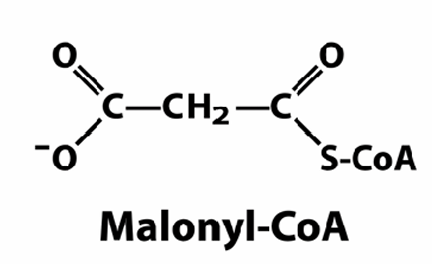
\includegraphics[width=0.25\linewidth]{Maloney.png}
    \caption{malonyl Co-A}
    \label{fig:enter-label}
\end{figure}
Malonyl Co-A is a \textbf{derivative of Acetyl-CoA produced in the cytosol} However acetyl-CoA is produced in the mitochontrial matrix so \textbf{Acteyl-CoA needs to be transported to the cytosol}:
\paragraph{transporting acetyl-CoA to cytosol}
\begin{figure}[H]
    \centering
    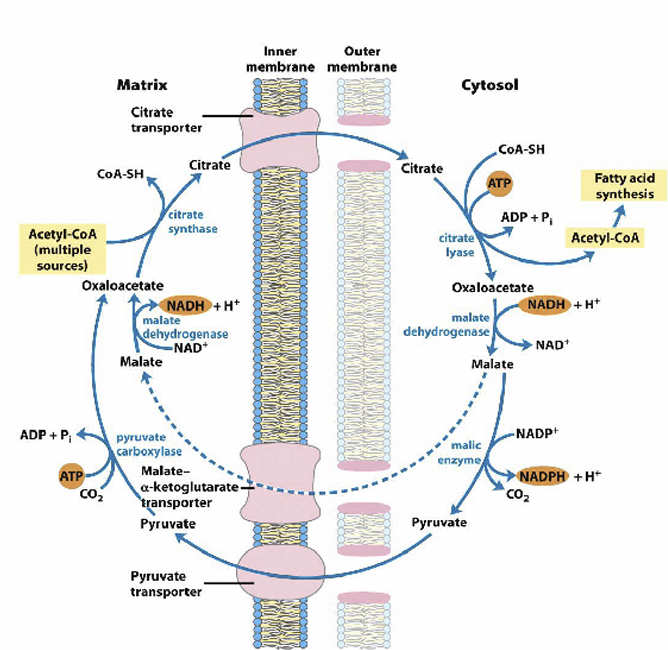
\includegraphics[width=0.6\linewidth]{actylCoA.png}
    \caption{Acetyl Co-A needs to be transported to cytosol}
    \label{fig:enter-label}
\end{figure}
\begin{enumerate}
    \item \textbf{oxaloactate and acteyl coA} are turned to citrate by \textbf{\gls{citratesynthase}}
    \item citrate can be transported across the membrane via \textbf{\gls{citrate_transporter}}
    \item citrate is turned to oxaloacetate and acetyl-CoA

    \item oxaloacetate is converted to malate by \textbf{Malate dehydrogenase} which in turn is turned to pyruvate by \textbf{\gls{malicenzyme}}. 
\end{enumerate}

step 4 is \textbf{crucial for generating NADPH} which will be used for FA sythesis later!

\paragraph{producing malonyl Co-A}
once acetyl-CoA has been transported into the cytosol malonyl coA can be synthesized. This steps involves a carboxylation of acetyl-CoA by \textbf{\gls{acetylcoacarboxylase}} and is the \textbf{rate limiting step of Fatty acid sythesis.}
\begin{figure}[H]
    \centering
    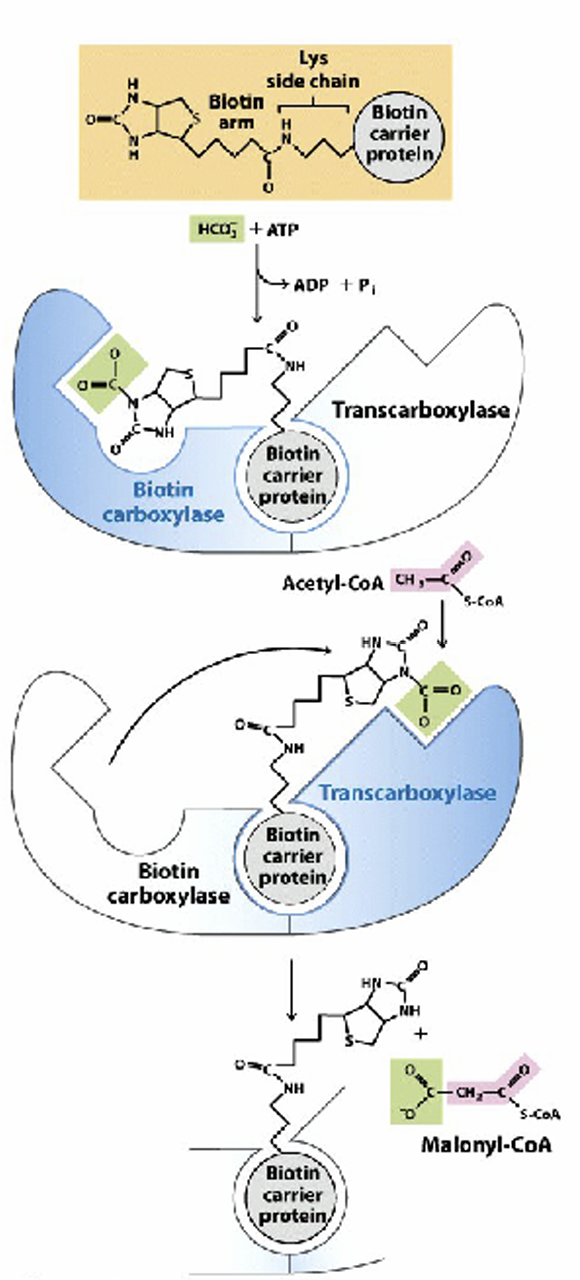
\includegraphics[width=0.3\linewidth]{Maloney_making.png}
    \caption{Malonyl sythesis}
    \label{fig:enter-label}
\end{figure}
A biotin carrier group which is part of \gls{acetylcoacarboxylase} is transiently carboxylated (with ATP consumtion) on a lysine - when in doubt lysine can do basically any PTM except phosphorylation .) - That then transfers the Co2 to acetyl-CoA turning it to malonyl-CoA.

\subsubsection{fatty acid sythase and it's domains overview}
\begin{figure}[H]
    \centering
    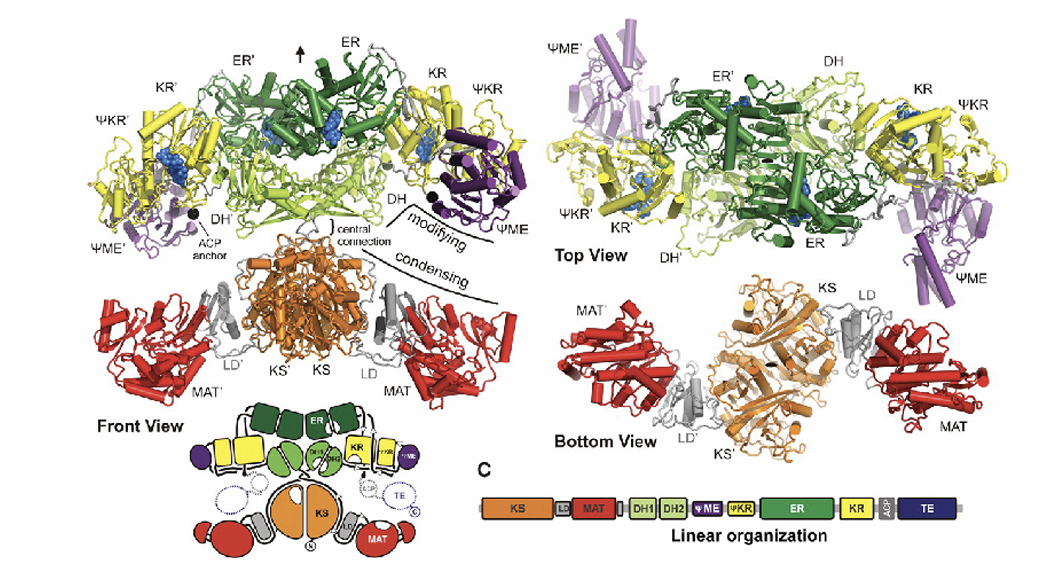
\includegraphics[width=0.5\linewidth]{FA_sythase.png}
    \caption{FA sythase structure and its domaines}
    \label{fig:enter-label}
\end{figure}
\textbf{\gls{FAsynthase}} is a huge multienzyme complex. The functional domains of \gls{FAsynthase} include:

\begin{itemize}
    \item \gls{BetaKetoacylSynthase} 
    \item \gls{MalonylAcetyltransferase} 
    \item \gls{AcylCarrierProtein}
    \item \gls{BetaKetoacylReductase} 
    \item \gls{Dehydratase}
    \item \gls{EnoylReductase} 
    \item \gls{Thioesterase} 
\end{itemize} 

\subsubsection{step by step mechanism}

bilanz:
\begin{figure}[H]
    \centering
    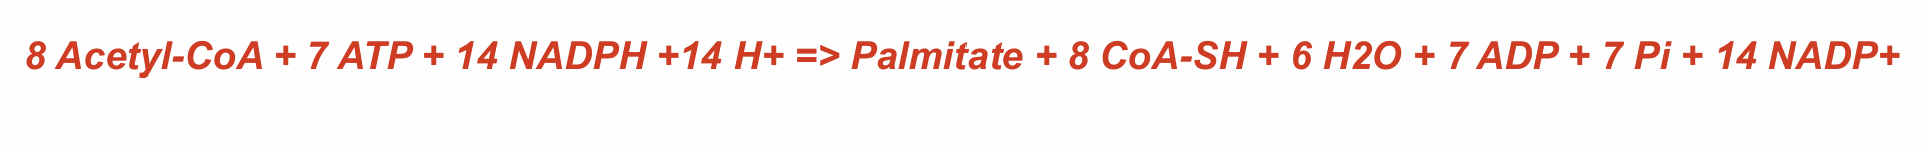
\includegraphics[width=1\linewidth]{bilanz.png}
    \caption{summary of what is used in palmitate sythesis}
    \label{fig:enter-label}
\end{figure}

\paragraph{step 0- loading}
\begin{figure}[H]
	\centering
	\subfigure[phase 1]{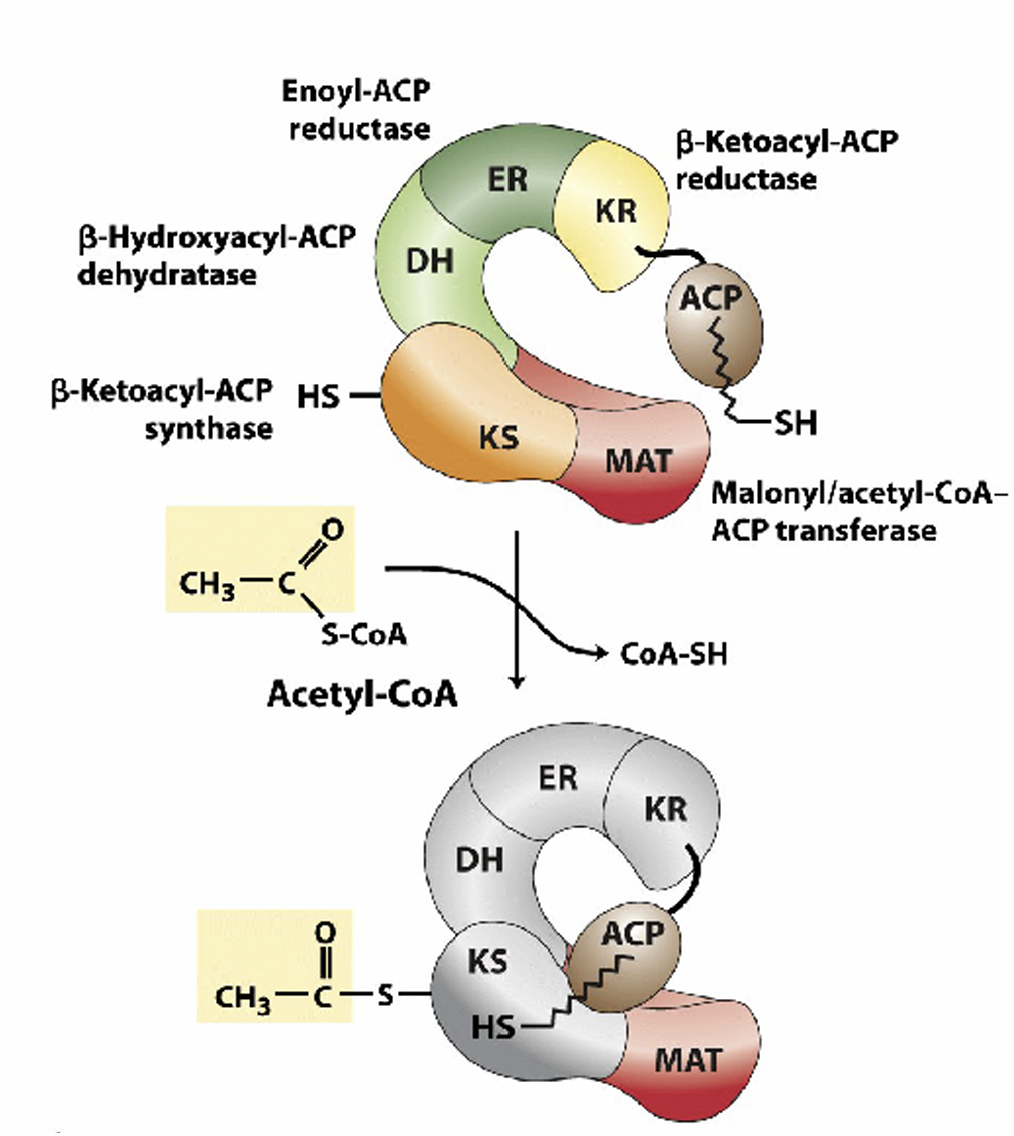
\includegraphics[width = 0.35 \textwidth]{loading_maloney.png}}
	\subfigure[phase 2]{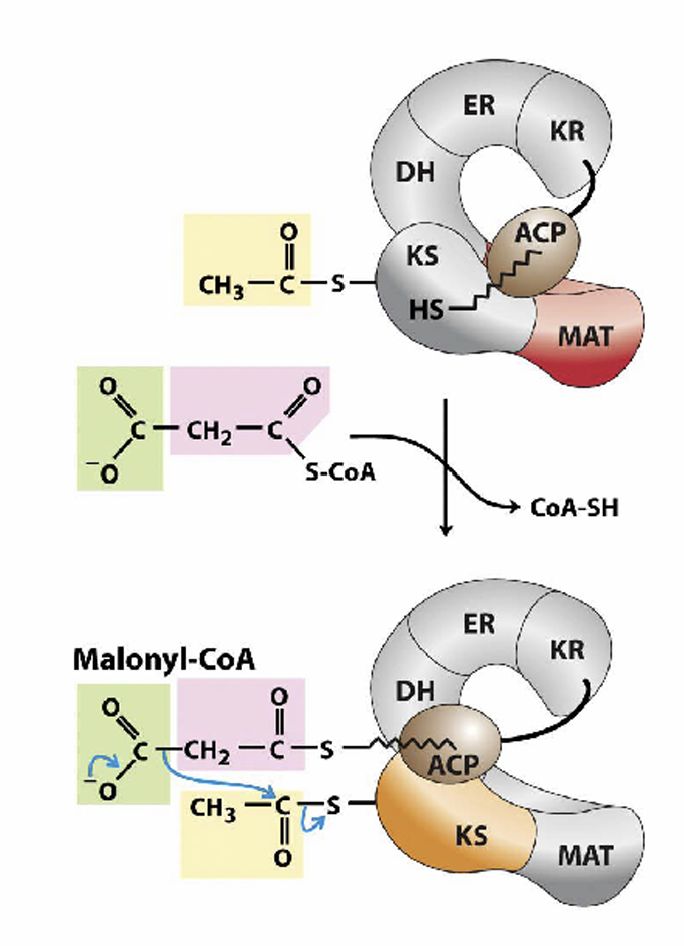
\includegraphics[width = 0.3\textwidth]{loadingmaloney.png}}
	\caption{loading step of FA sythesis}
\end{figure}


\begin{enumerate}
    \item \textbf{phase 1:} acetyl-CoA  molecule is 
    condensed to a \textbf{Cys} residue in the \textbf{\gls{BetaKetoacylSynthase}} domain. To do this it is\textbf{ first loaded onto \gls{AcylCarrierProtein}} then \textbf{transfered to KS domain}. This is catalyzed by \textbf{\gls{MalonylAcetyltransferase}}

    \item \textbf{phase 2:} Malonyl-CaA is added to \textbf{\gls{AcylCarrierProtein}}. where it is close to acetyl coA and ready to react.
\end{enumerate}


\paragraph{step 1 - condensation}
\begin{figure}[H]
    \centering
    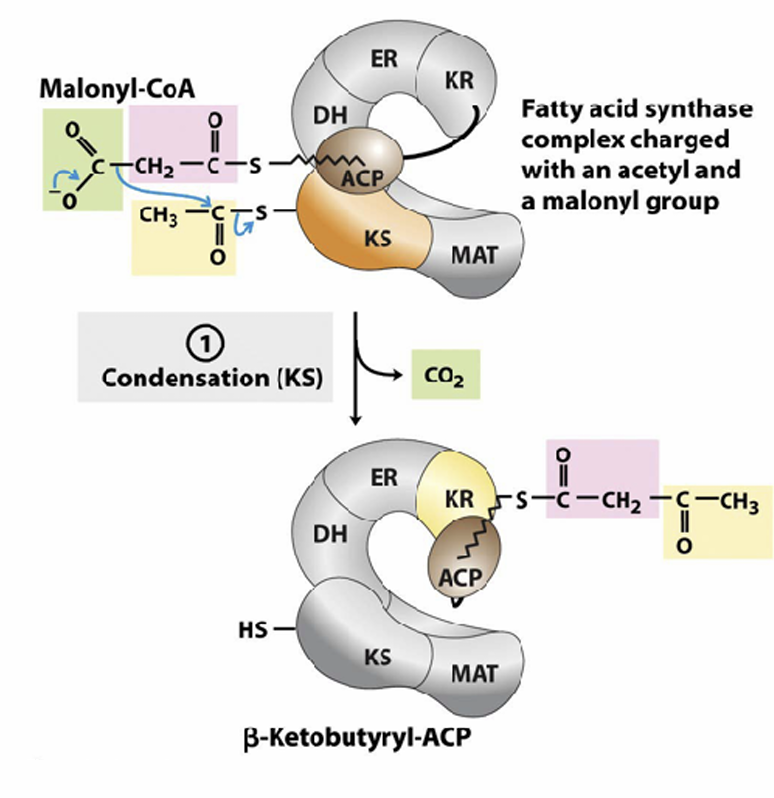
\includegraphics[width=0.5\linewidth]{condensation.png}
    \caption{condensation step}
    \label{fig:enter-label}
\end{figure}

In this step Malonyl and Acetyl are condensed to \textbf{\gls{acetoacetyl}}, with the \textbf{release of Co2}. This reaction is catalyzed by \textbf{\gls{BetaKetoacylSynthase}}. Facts to know:
\begin{enumerate}
    \item this is the energetically driving step of FA sythesis
    \item co2 release is the same one that was originally added by acetyl-coA carboxylase.
    \item this reaction is exergonic.
    \item reaction is similar to  PEP-carboxykinase in gluconeogensis.
\end{enumerate}

\paragraph{step 2 - reduction}
\begin{figure}[H]
    \centering
    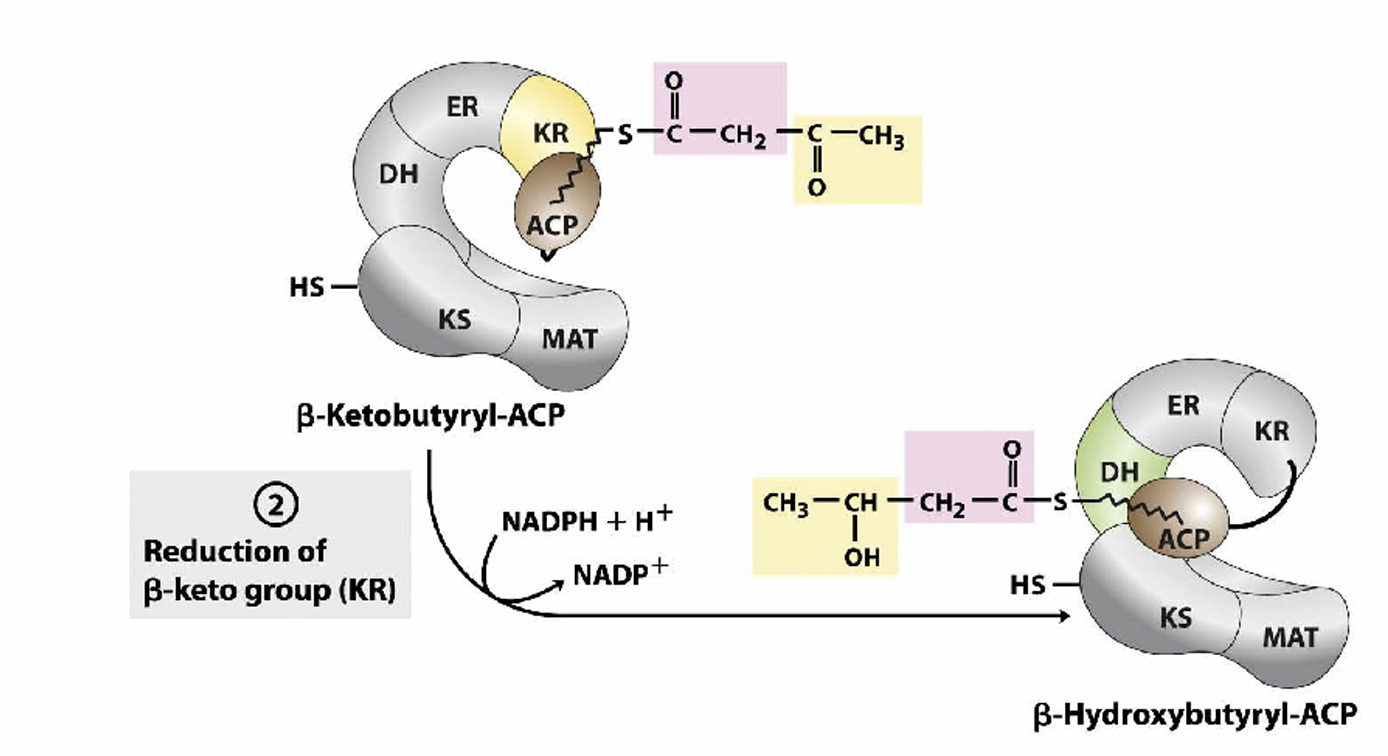
\includegraphics[width=0.5\linewidth]{step2.png}
    \caption{reduction step}
    \label{fig:enter-label}
\end{figure}
 In the second step (reduction) acetoacetyl-ACP is \textbf{reduced to \gls{bhbcoa}} by 
the \textbf{\gls{BetaKetoacylReductase}} with oxidation of one NADPH molecule.


\paragraph{step 3 - dehydration}
\begin{figure}[H]
    \centering
    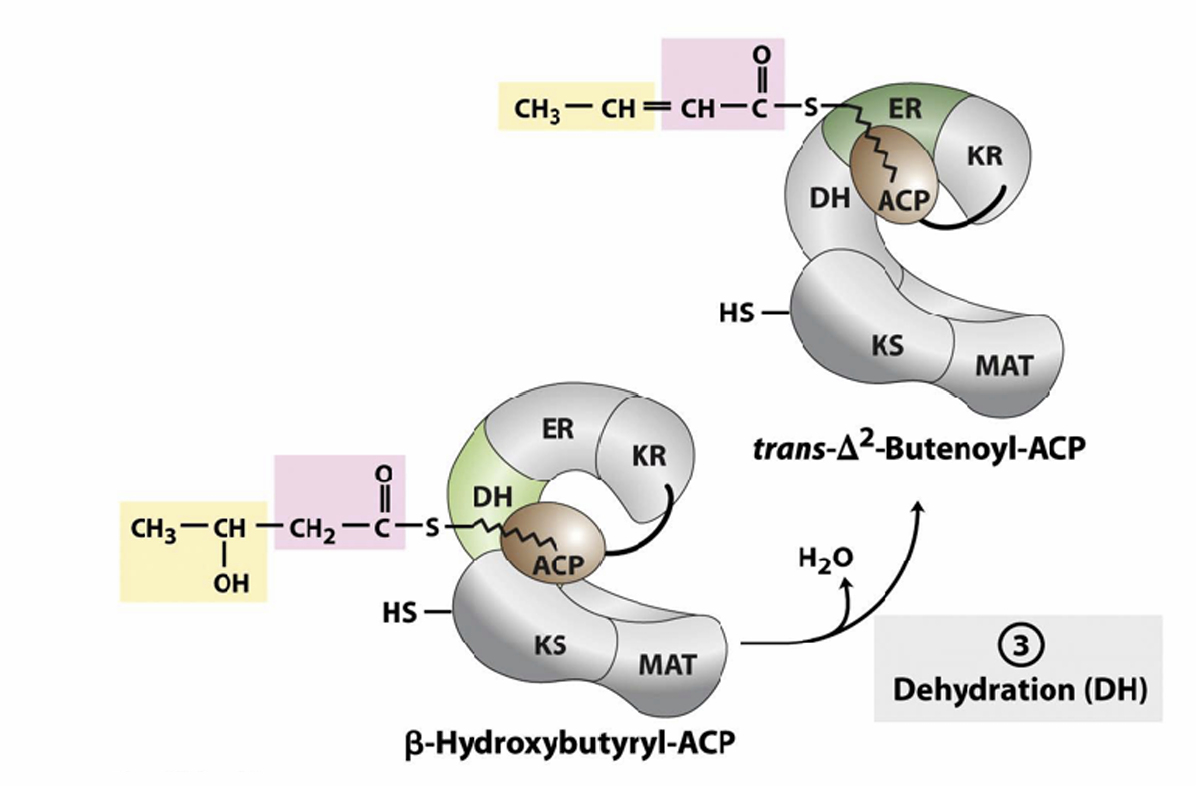
\includegraphics[width=0.5\linewidth]{step3.png}
    \caption{dehydration step}
    \label{fig:enter-label}
\end{figure}

\textbf{\gls{bhbcoa}} \textbf{loses a H2O }molecule to yield \textbf{\gls{transD2ButenoylACP}} in a reaction catalysed by the \textbf{\gls{Dehydratase}}

\paragraph{step 4 - reduction}
\begin{figure}[H]
    \centering
    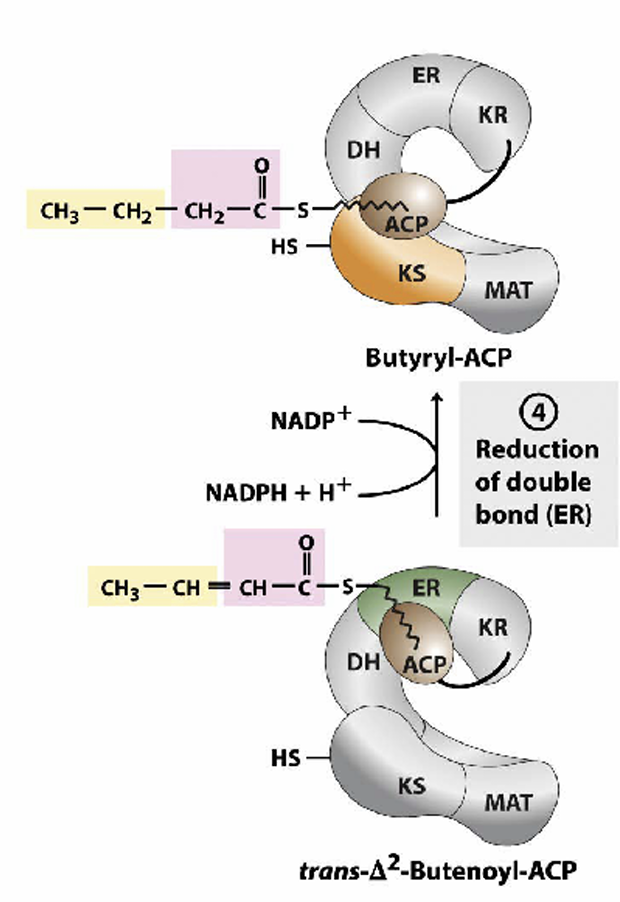
\includegraphics[width=0.3\linewidth]{step4.png}
    \caption{2nd.reduction step}
    \label{fig:enter-label}
\end{figure}

\textbf{\gls{transD2ButenoylACP}} is reduced to \textbf{\gls{butyrylACP}} in a reaction catalyzed by the \gls{EnoylReductase} where the double bond C2 / C3 is reduced and a
molecule of NADPH is oxidized. 

--> \textbf{here we have elongated acetate-ACP (2C fatty acid) into butyrylACP (4C fatty acid)}

\paragraph{step 5 - translocation }
\begin{figure}[H]
    \centering
    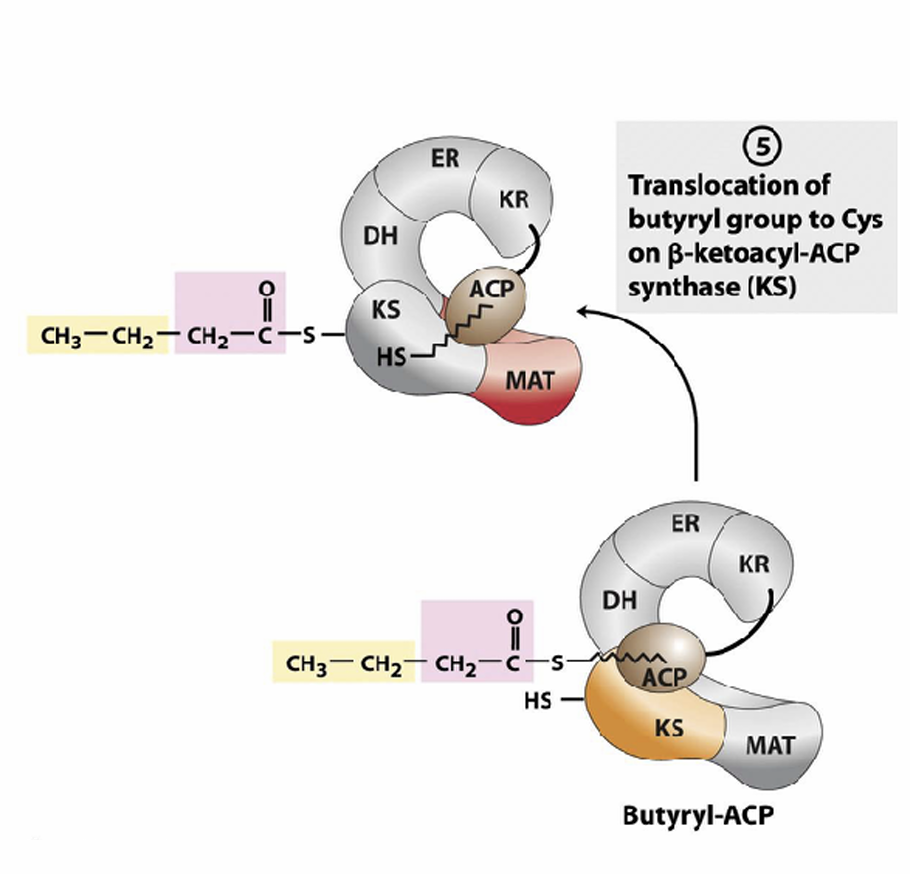
\includegraphics[width=0.5\linewidth]{step5.png}
    \caption{translocation of butaryl (or another FA) onto KS domain}
    \label{fig:enter-label}
\end{figure}

 To start a new cycle it 
needs to be transferred from the 
ACP to the Cys residue of the \textbf{\gls{BetaKetoacylSynthase}}. This step is very similar to step one with one important difference. The \textbf{ACP domain only accepts malonyl and acetyl so larger FA stay on the KS domain}

\paragraph{step 6 - reload a malonyl}
\begin{figure}[H]
    \centering
    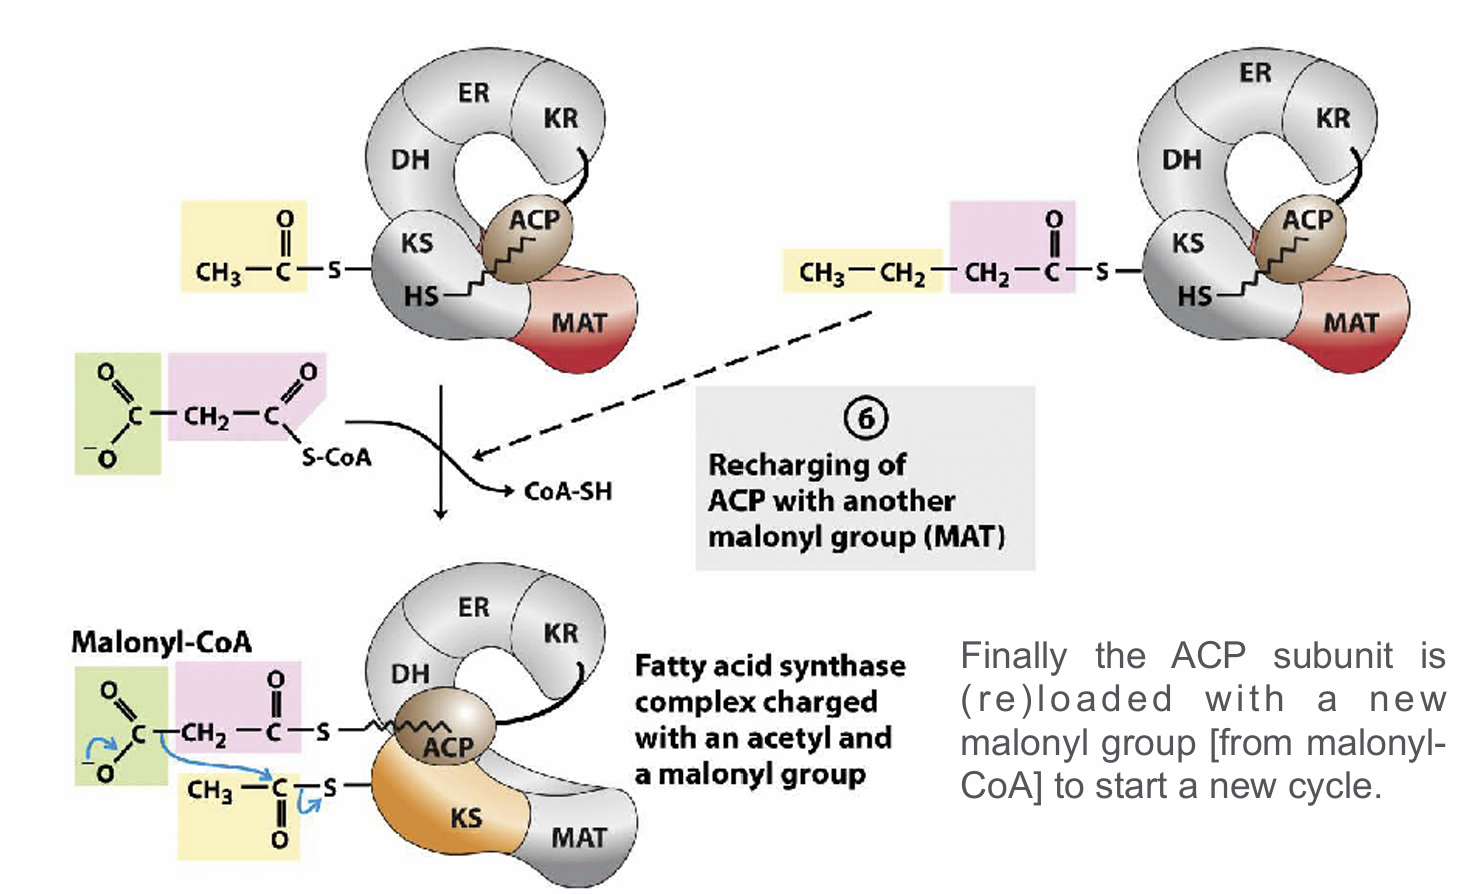
\includegraphics[width=0.5\linewidth]{step6.png}
    \caption{reloading a malonyl}
    \label{fig:enter-label}
\end{figure}
This step is \textbf{identical to step one} except that there is no need to translocate Acetyl to KS domain. And now butaryl is in the place of acetyl.

\subsubsection{useful for C-labelling shit}
\begin{figure}[H]
    \centering
    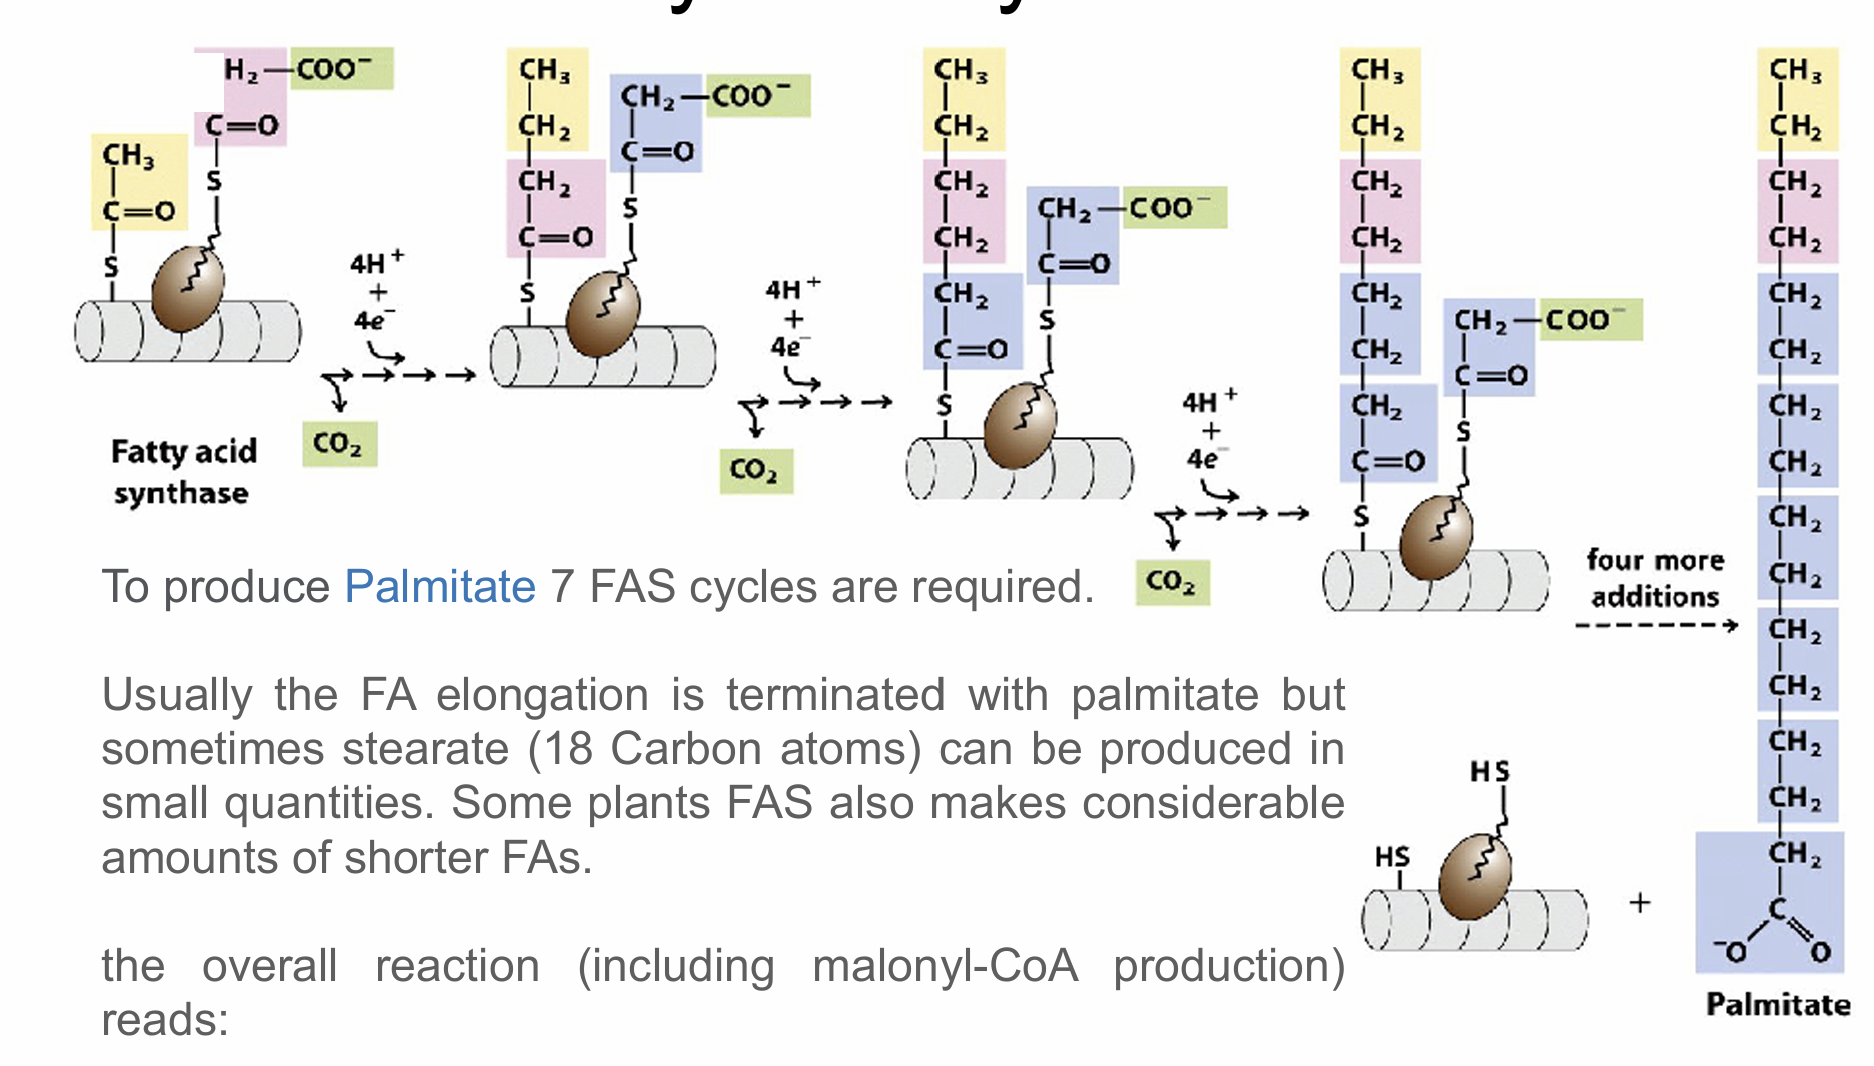
\includegraphics[width=\linewidth]{overviewPalmitate.png}
    \caption{overview of palmitate carbons}
    \label{fig:enter-label}
\end{figure}


\subsubsection{palmitate as precursor and making other FA}
Palmitate is the main FA produced via this pathway. It consists of 16C so will take \textbf{7 cyles to produce} (7*2 + 2C from acetyl). Longer Fatty acids can be produced by elongating plamitate via the same process. The \textbf{fatty acid elongation systems} are located in the endoplasmatic reticulum and mitochondria. Moreover, \textbf{double bonds} can also be introduced to produce unsaturated fatty acids.
\begin{figure}[H]
    \centering
    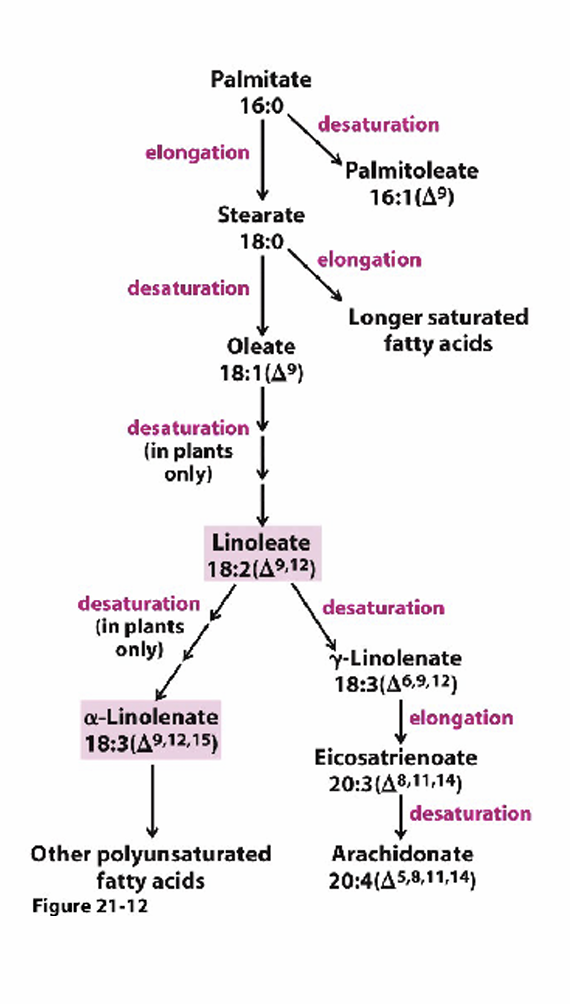
\includegraphics[width=0.5\linewidth]{palmitate_stuff.png}
    \caption{making other FA from plamitate as precursor}
    \label{fig:enter-label}
\end{figure}
\paragraph{introducing Double bonds}
\begin{figure}[H]
    \centering
    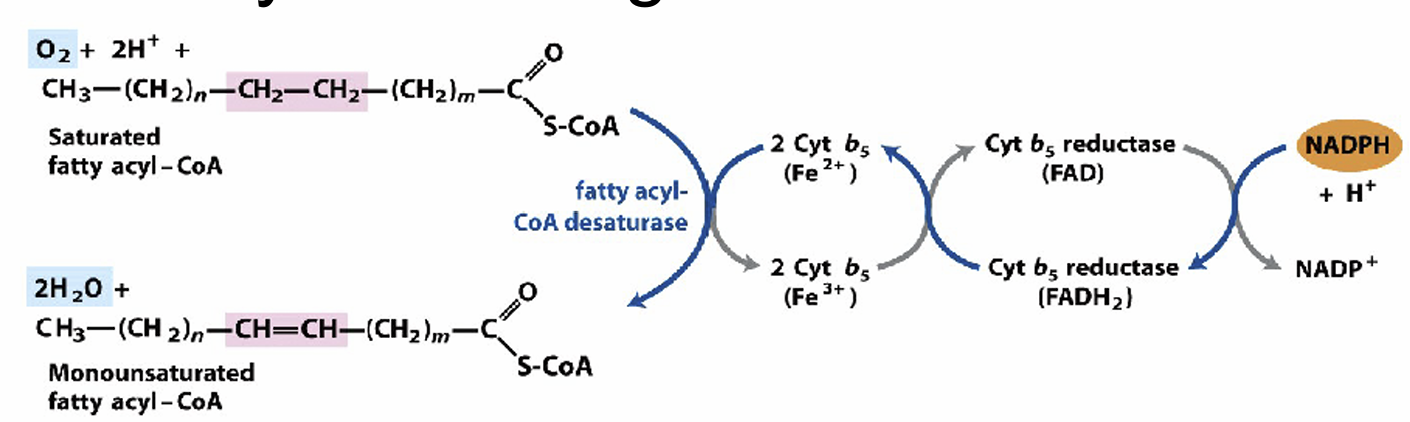
\includegraphics[width=1\linewidth]{DBonds.png}
    \caption{introducing double bonds}
    \label{fig:enter-label}
\end{figure}
acyl co-As such as palimatate can be desturated by \textbf{\gls{fattyAcylCoADesaturase}} Which transfers 2 electrons from NADPH (oxidation) to create the double bond. This takes place \textbf{in the ER of liver cells}. Not all unsaturated acids can be produced though.\textbf{ Mammals will only produce $\Delta^9$ fatty acids}, however some plants can produce $\Delta^{9,12}$ and $\Delta^{9,12,15}$ fatty acids. For mammals these are thus essential Fatty acids!\\
\indent \textbf{Attention Confusion:} Oxygen (not shown) is reduced to H2O, both the fatty acid and the iron is oxidized

\subsection{Phosphatidic acid sythesis}
\begin{figure}[H]
    \centering
    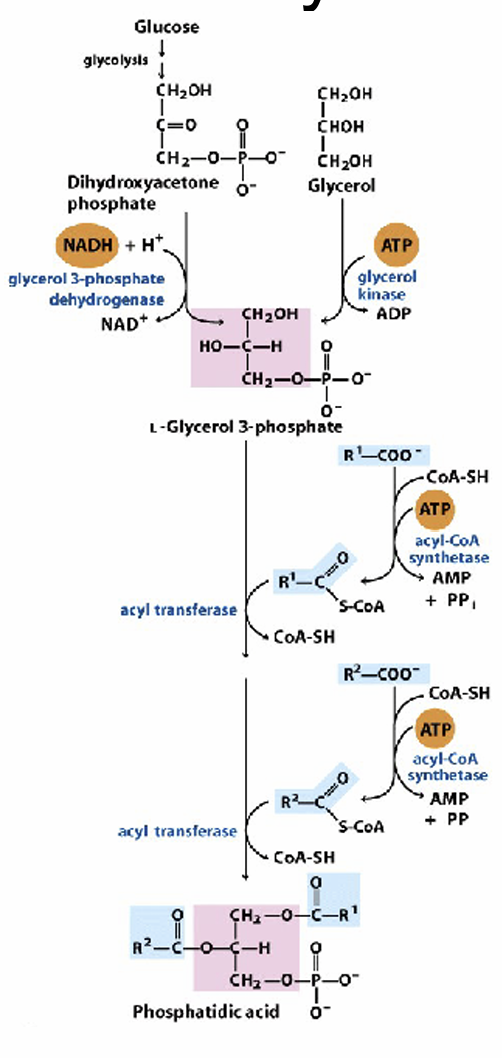
\includegraphics[width=0.25\linewidth]{phosphatidicAcid.png}
    \caption{phosphatidic acid(PtAC) sythesis}
    \label{fig:enter-label}
\end{figure}
\textbf{\gls{phosphatidicacid}} is used for the synthesis of triglycerides (TAGs) and glycerophospholipids. therefore it is an important precursor for various lipids. 
\begin{enumerate}
    \item \textbf{generate Glycerol-3-phosphate}
    \begin{enumerate}
        \item \textbf{from glycolisis:} Dehydroxyacetonphosphate (\textbf{DHAP}) can be converted by \textbf{\gls{glycerol3phosphateDehydrogenase}} into glycerol-3-phosphate.

        \item \textbf{Phosphorylation of glycerol:} kidney cells have \textbf{\gls{glycerolKinase}} that can directly phosphorylate glycerol.
    \end{enumerate}
    \item \textbf{generate Acly-CoA:} Acyl-CoAs are formed from fatty acids by the action of the enzyme \textbf{\gls{acylCoASynthetase}} (this is the same molecule that activates fatty acids for their entry into beta-oxydation to catalyze the reaction).

    \item \textbf{\gls{acylTransferases}} esterify acyl chains in positions C-1 and C-2 of the Glycerol-3-Phosphate to produce phosphatidic acid.
\end{enumerate}


\subsection{triglyceride sythesis}
\begin{figure}[H]
    \centering
    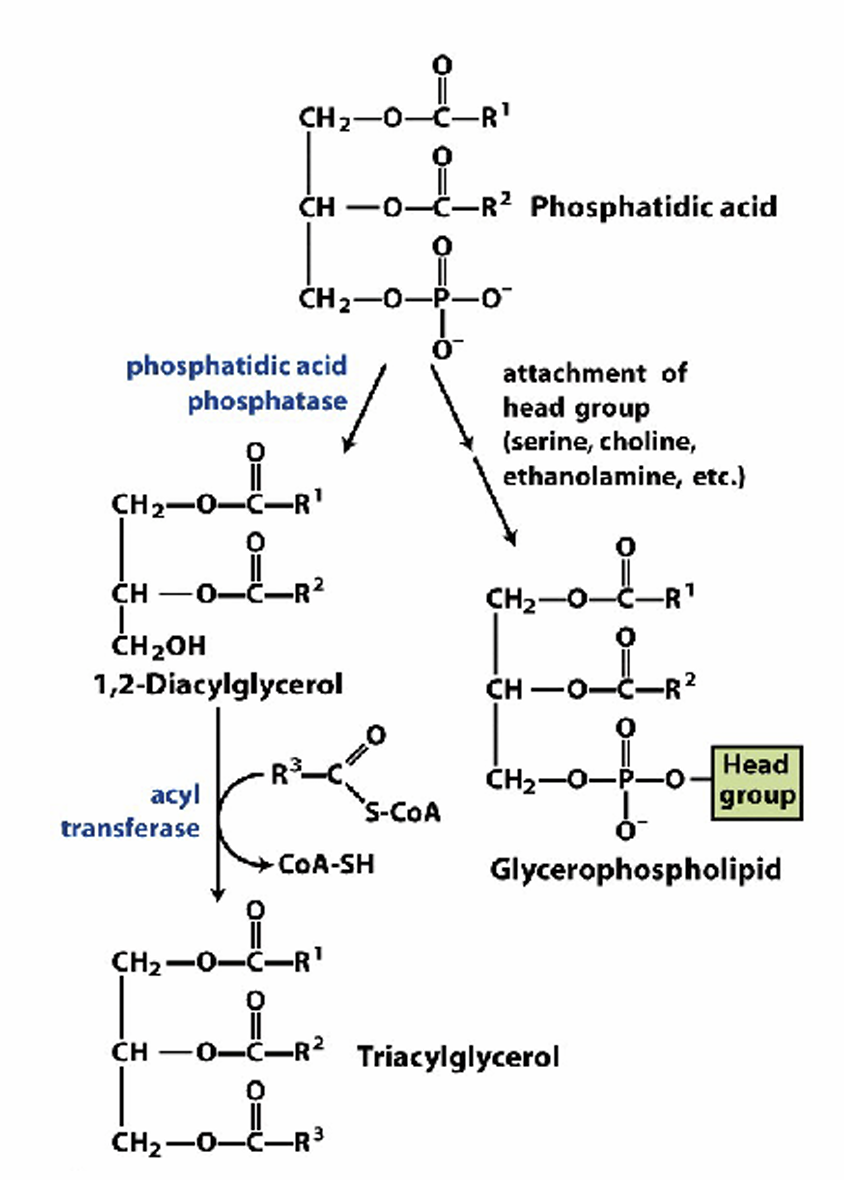
\includegraphics[width=0.4\linewidth]{TAG_syth.png}
    \caption{triglyceride synthesis}
    \label{fig:enter-label}
\end{figure}
\begin{enumerate}
    \item phosphatidic acid is dephosphorylated to form diacylglycerol by \textbf{\gls{phosphatidicacidphosphatase}}
    
    \item \gls{acylTransferases} that catalyse the esterification of a third fatty acid to glycerol (in position C-3).
\end{enumerate}


\subsection{Glycerophospholipids sythesis}
\begin{figure}[H]
    \centering
    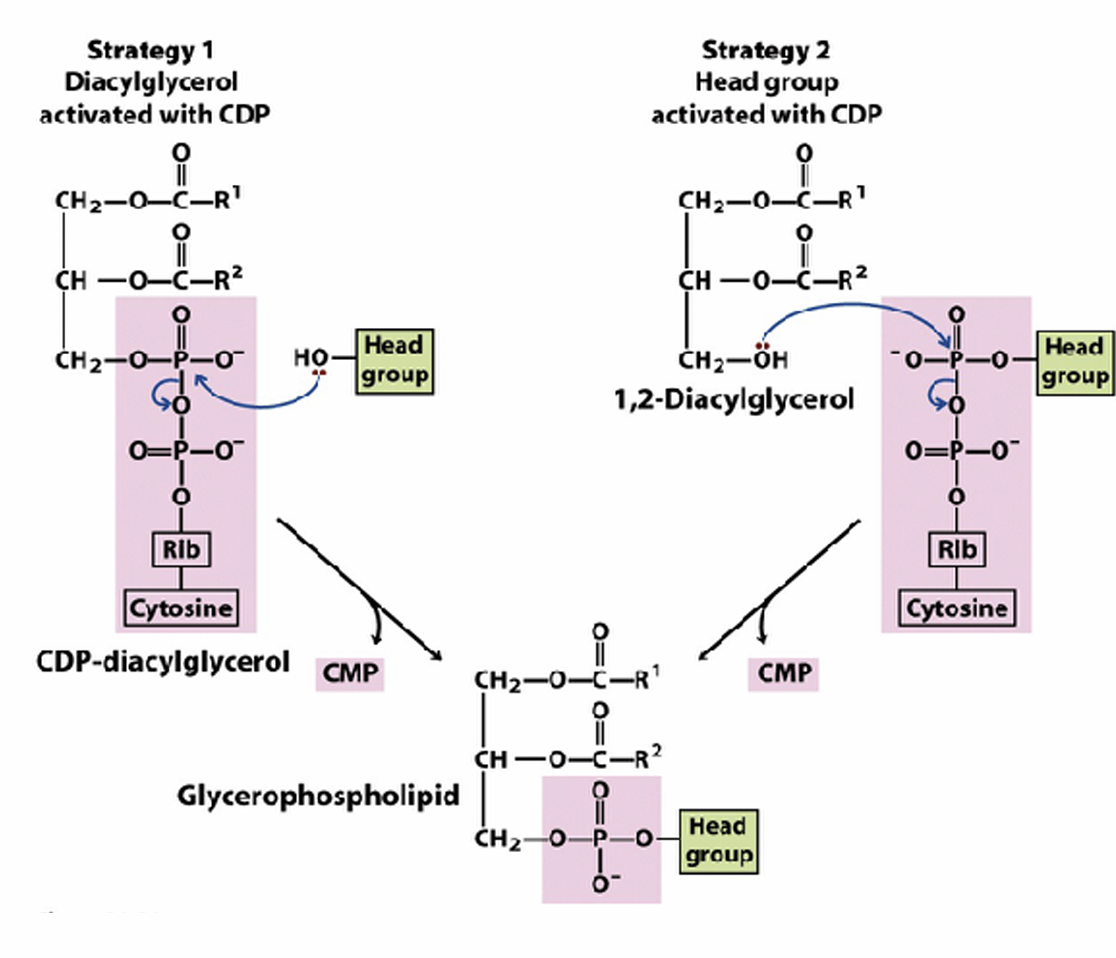
\includegraphics[width=0.5\linewidth]{glycerophospholipid.png}
    \caption{glycerophospholipid sythesis}
    \label{fig:enter-label}
\end{figure}
There are two strategies for creating glycerophospholipids depending on which precursor is activated using cmp:
\begin{enumerate}
    \item \textbf{strategy 1 - ptAc activation:} This consists in the activation of phosphatidic acid(ptAC) to form \textbf{CDP-diacylglycerol.}

    \item \textbf{strategy 2 - head group activation:} Here instead of activating ptAc, the head group is activated using CMP.
\end{enumerate}

In either case after the\textbf{ condenstaion of the head group and the ptAC lead to release of CMP}

\subsubsection{bacterial glycerophospholipid sythesis}
\begin{figure}[H]
    \centering
    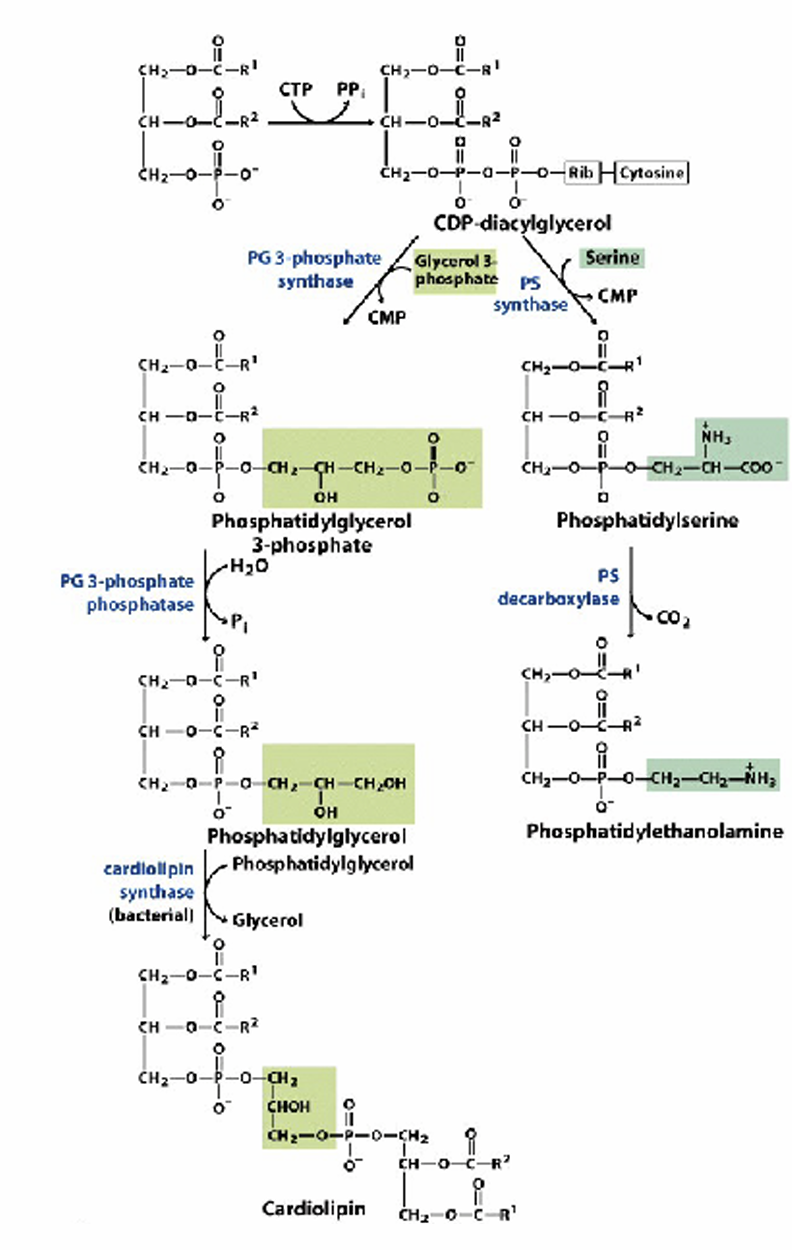
\includegraphics[width=0.5\linewidth]{bacteria_lipids.png}
    \caption{bacteria can make most glycerophospholipids via strategy 1}
    \label{fig:enter-label}
\end{figure}
In E. coli almost \textbf{all glycerophospholipids can be obtained using strategy 1}
\begin{itemize}
    \item phosphatydilSer (\textbf{ptdSer}): strategy 1
    \item phosphatidylglycerol-3-phosphate (\textbf{ptdGly(3)p}): strategy 1
    \item phosphatidylethanolamine (\textbf{PtdEtn}): decarboxylation of ptdSer
    \item \textbf{PtdGly}: dephosphorylation of ptdGly(3)p
    \item \textbf{cardiolipin}: condesation of two pdtGly molecules
\end{itemize}
   

\subsubsection{eucaryotic glycerophospholipid sythesis}
\begin{figure}[H]
	\centering
	\subfigure[glycerophospholipid production in eukaryotes via strategy 1]{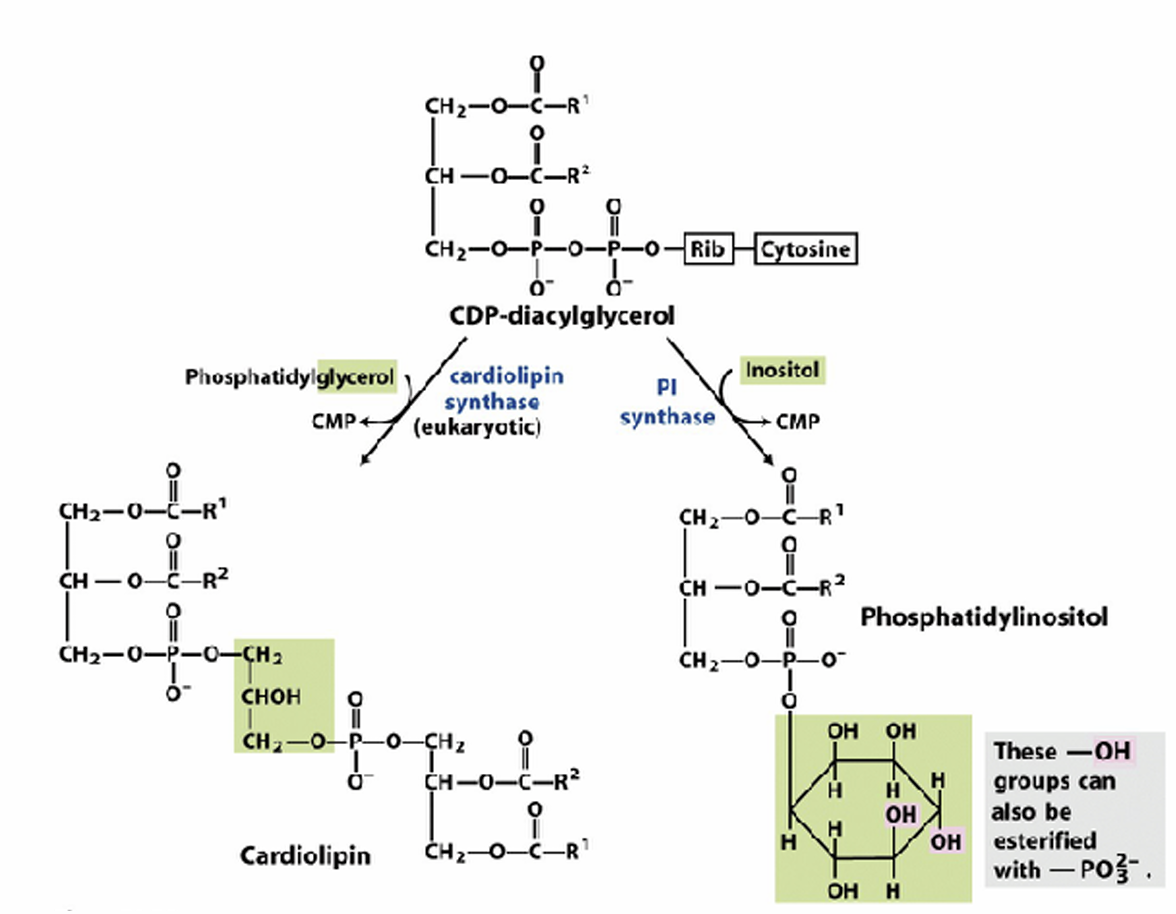
\includegraphics[width = 0.6 \textwidth]{eukaryoticlipids.png}}
	\subfigure[ptdCho sythesis in eukaryotes]{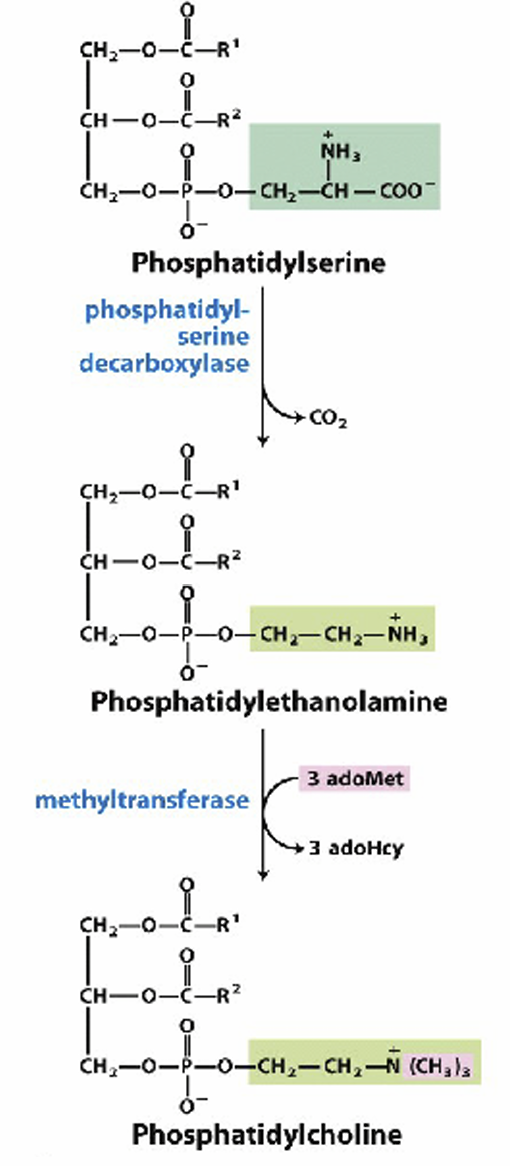
\includegraphics[width = 0.2\textwidth]{ptdCho.png}}
	\caption{loading step of FA sythesis}
\end{figure}


\begin{itemize}
    \item \textbf{PtdIns}: strategy 1 using \textbf{\gls{phosphatidylinositol_synthase}}
     \item \textbf{PtdGly}: dephosphorylation of ptdGly(3)p
    
    \item \textbf{cardiolipin}: CDP-diacylglycerol is used to produce cardiolipin similar to E. coli but only one ptdGly is used.

    \item \textbf{ptdSer}: strategy 1 (for yeast, not for mammals) or head group exchange between PtdSer and PtdEtn (mammals do it like this instead)
    \item phosphatidylcholine (\textbf{ptdCho}): addition of three methyl groups to the 
    PtdEtn amine group operated by a methyltransferase. (this is for yeast. for mammels see section 1.4.2.1)
    \item (for mammals) \textbf{amine containg glycerophospholipids} (ptdCho, ptdEtn): strategy 2 
\end{itemize}
\paragraph{phosphatidylinositol sythesis}
\begin{figure}[H]
    \centering
    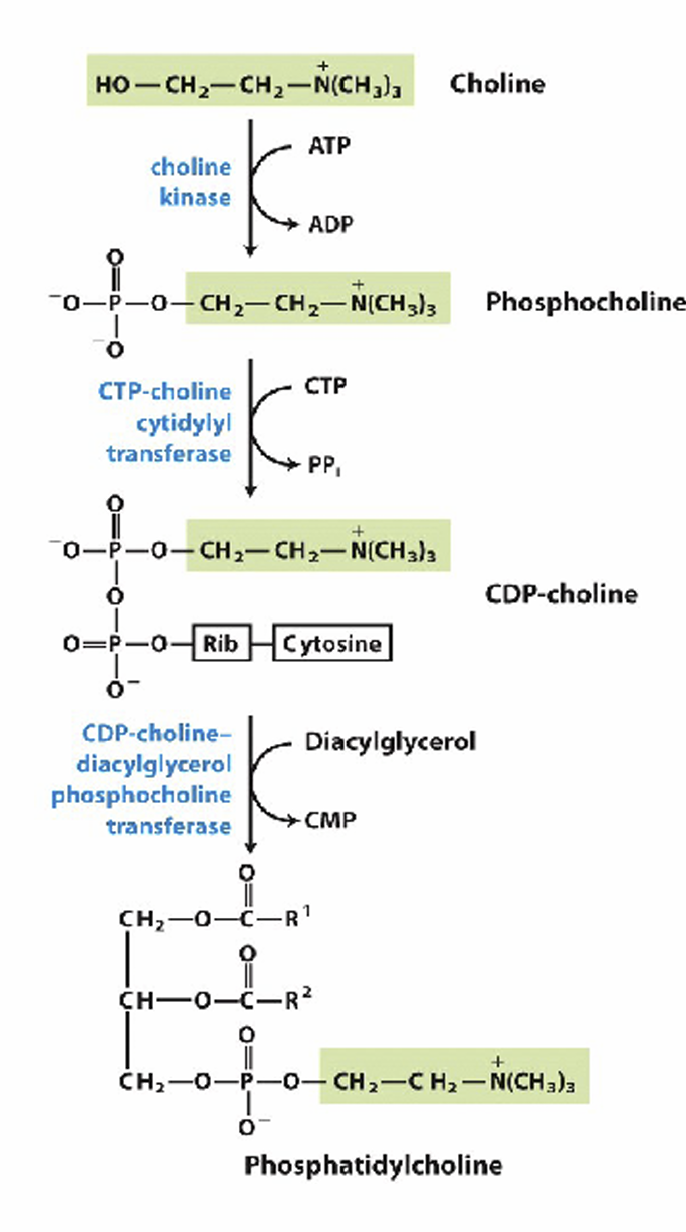
\includegraphics[width=0.5\linewidth]{ptdChomammals.png}
    \caption{ptdCho sythesis in mammals}
    \label{fig:enter-label}
\end{figure}
mammals sythesis ptCho via strategy 2 as follows:
\begin{enumerate}
    \item choline is phosphorylated by \textbf{\gls{choline_kinase} }to 
phosphocholine  
    \item phosphocholine is complexed to CDP to form 
    CDP-choline by CTP-choline cytidylyl 
    transferase \textbf{\gls{ctp_choline_cytidylyltransferase}}
    \item  CDP-choline is condensed to diacylglycerol to 
produce PtdCho by the action of \textbf{\gls{cdp_choline_dag_phosphocholine_transferase}}
\end{enumerate}

\subsection{Cholesterol sythesis}

\begin{figure}[H]
	\centering
	\subfigure[Cholesterol and it's precursors]{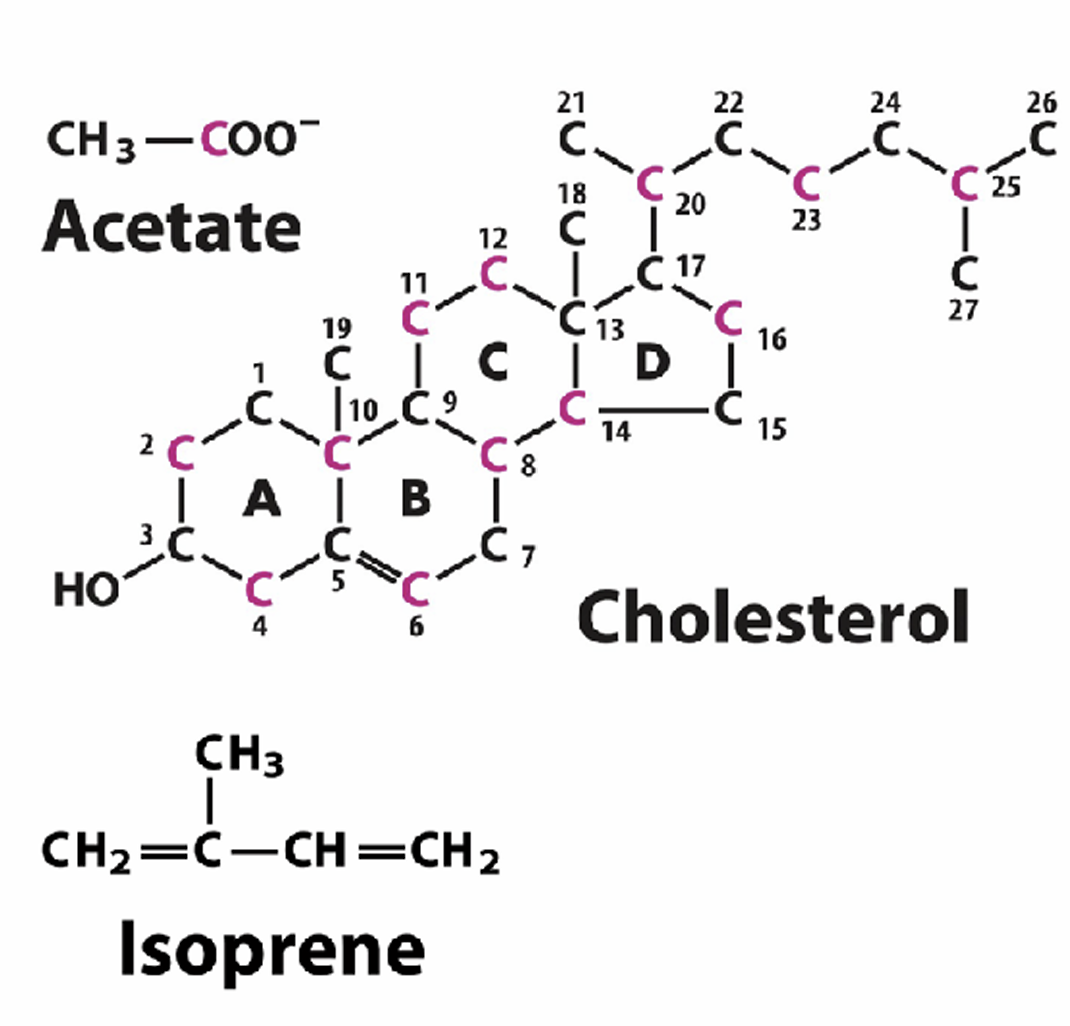
\includegraphics[width = 0.4 \textwidth]{cholesterolOverview.png}}
	\subfigure[sythesis overview]{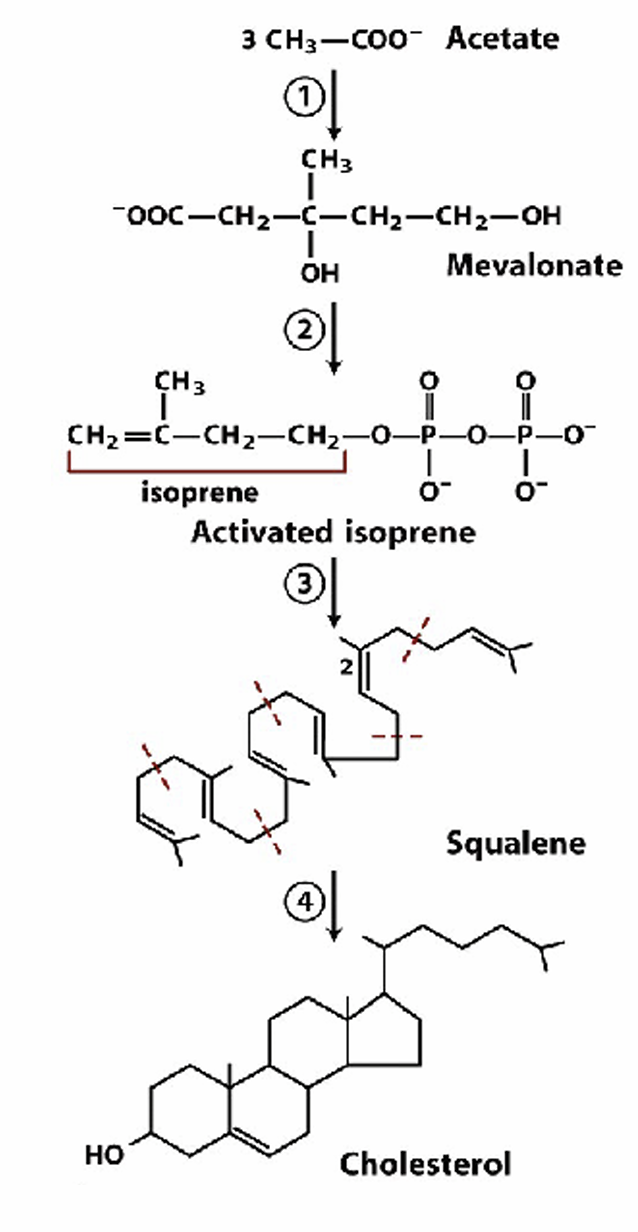
\includegraphics[width = 0.3\textwidth]{melvalonate.png}}
	\caption{cholesterol sythesis}
\end{figure}



Cholesterol is formed in a 4 step pathway: 
\begin{enumerate}
    \item  3 Acetyl groups are condensed to form 
\textbf{mevalonate}
\item Mevalonate is converted into \textbf{activated 
isoprene }
\item 6 \gls{isoprene} units are polymerised into 
\textbf{squalene}
\item \gls{squalene} is converted to cholesterol.
\end{enumerate}

\subsubsection{step 1 - melvalonate sythesis}
\begin{figure}[H]
    \centering
    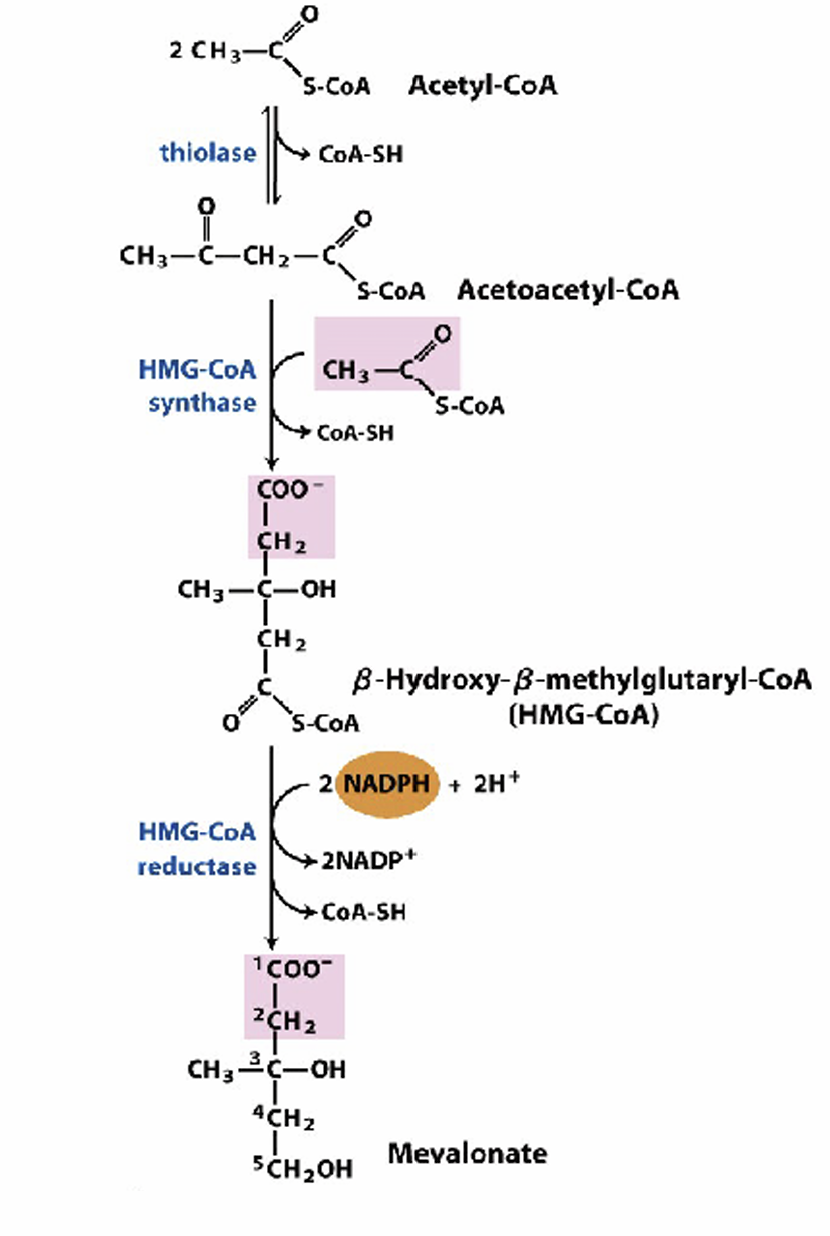
\includegraphics[width=0.5\linewidth]{melvalonateSythesis.png}
    \caption{\gls{mevalonate} sythesis}
    \label{fig:enter-label}
\end{figure}
\begin{enumerate}
    \item Two acetyl-CoA molecules are condensed to form \textbf{acetoacetyl-CoA} by \textbf{\gls{thiolase}}.
    
    \item \textbf{\gls{acetoacetyl}-CoA} is further condensed with another acetyl-CoA molecule to produce $\beta$-hydroxy-$\beta$-methylglutaryl-CoA \textbf{(HMG-CoA)} by \textbf{\gls{hmg_coa_synthase}}.
    
    \item $\beta$-hydroxy-$\beta$-methylglutaryl-CoA is reduced to \textit{mevalonate} by \textbf{HMG-CoA reductase} (Integral ER membrane protein). This is the \textbf{committing step}.
\end{enumerate}


\subsubsection{step 2 - isoprene sythesis}

\begin{figure}[H]
    \centering
    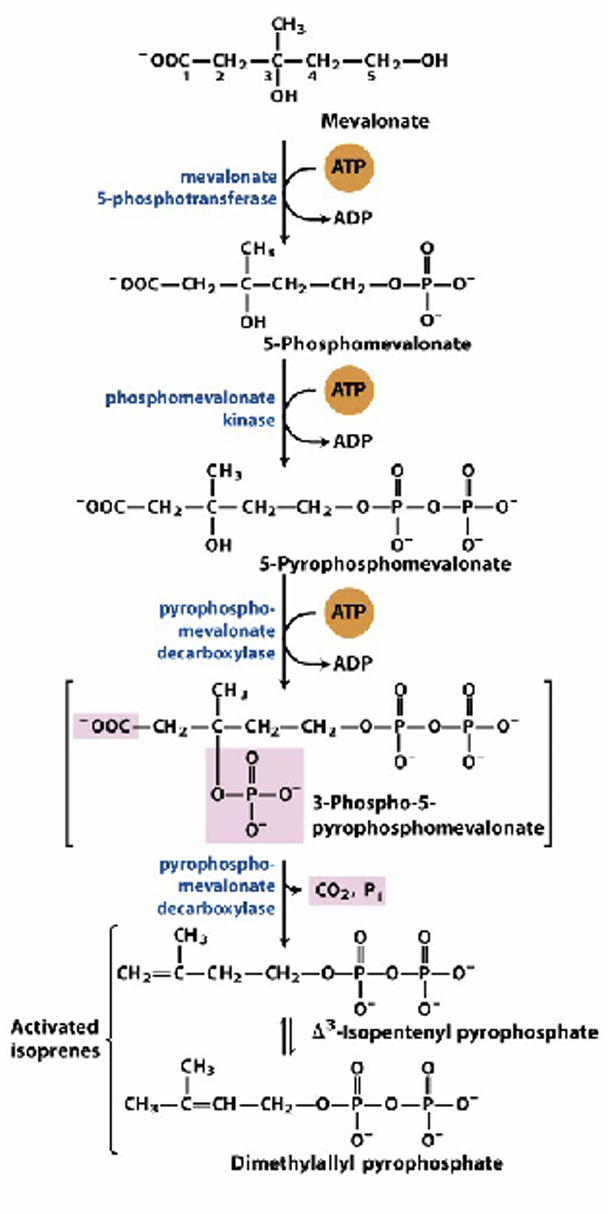
\includegraphics[width=0.4\linewidth]{isopreneSythesis.png}
    \caption{isoprene sythesis}
    \label{fig:enter-label}
\end{figure}
\begin{enumerate}
    \item Mevalonate is phosphorylated by \textbf{\gls{mevalonate_5_phosphotransferase} }to form \textbf{5-phosphomevalonate}.
    
    \item 5-phosphomevalonate is phosphorylated by \textbf{\gls{phosphomevalonate_kinase}} to produce \textbf{5-pyrophosphomevalonate}.
    
    \item 5-pyrophosphomevalonate is phosphorylated to \textbf{3-phospho-5-pyrophosphomevalonate} by \textbf{\gls{pyrophosphomevalonate_decarboxylase}.}
    
    \item The same enzyme, \textbf{\gls{pyrophosphomevalonate_decarboxylase}}, catalyzes the decarboxylation of 3-phospho-5-pyrophosphomevalonate to produce activated isoprene units (Isopentyl pyrophophate  (IPP) and dimethylallyl pyrophosphate.)
\end{enumerate}


\subsubsection{step 3 - squalene sythesis}
\begin{figure}[H]
    \centering
    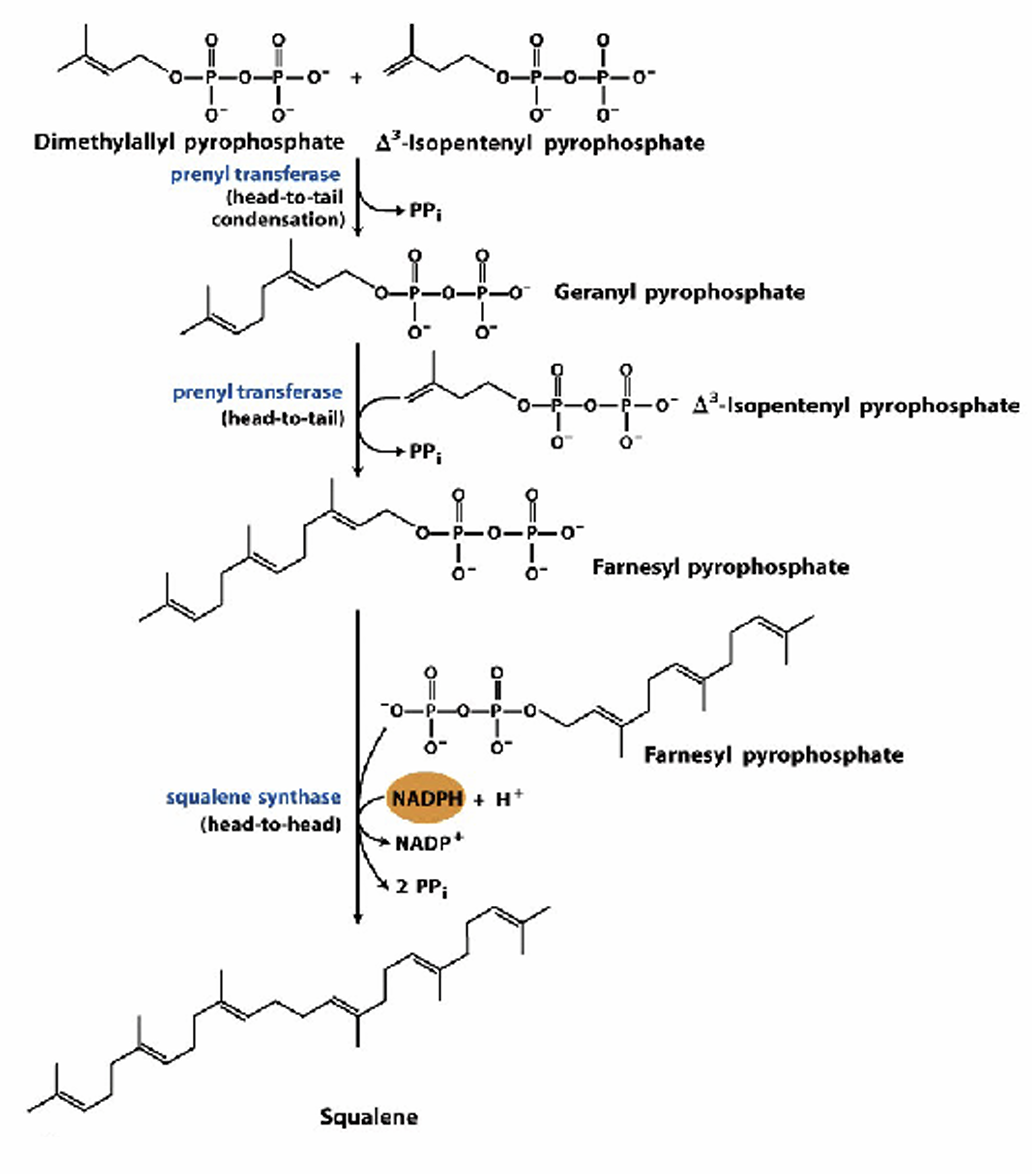
\includegraphics[width=0.5\linewidth]{squaleneSythesis.png}
    \caption{squalene sythesis}
    \label{fig:enter-label}
\end{figure}


\begin{enumerate}
    \item \textbf{\gls{isopentenyl_pp}} and \textbf{\gls{dimethylallyl_pp}} (isoprene units) undergo a \textbf{head-to-tail} condensation to form \textbf{\gls{geranyl_pp}}, catalyzed by the enzyme \textbf{\gls{prenyl_transferase}.}
    
    \item Geranyl pyrophosphate and isopentenyl pyrophosphate undergo another head-to-tail condensation to form \textbf{\gls{farnesyl_pp}}, also catalyzed by \textbf{\gls{prenyl_transferase}.}
    
    \item Two farnesyl pyrophosphate molecules are condensed \textbf{head-to-head} to form \textbf{\gls{squalene}}, catalyzed by \textbf{\gls{squalene_synthase}.}
\end{enumerate}
\subsubsection{step 4 - ring closure}
\begin{figure}[H]
    \centering
    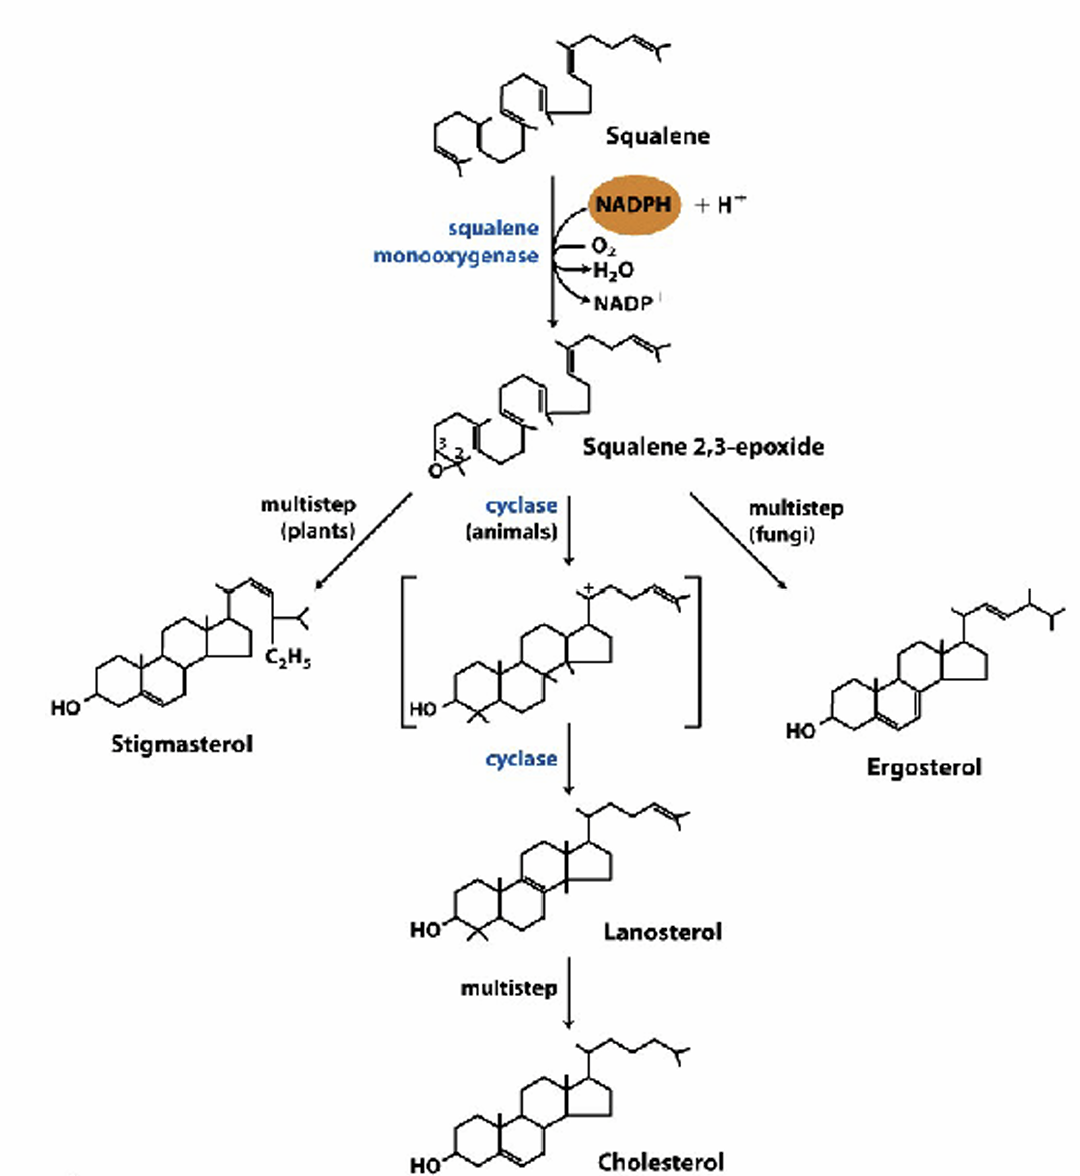
\includegraphics[width=0.5\linewidth]{ringClosure.png}
    \caption{ring closure and final step of cholesterol sythesis}
    \label{fig:enter-label}
\end{figure}
\begin{enumerate}
    \item \gls{squalene} is oxygenated by \textbf{\gls{squalene_monooxygenase}} to form \textbf{\gls{squalene_epoxide}}. 
    \item Cyclization reactions then convert squalene 2,3-epoxide into\textbf{ \gls{lanosterol}}, which, through a complex series of about 20 reactions, is ultimately converted into \gls{cholesterol}.
\end{enumerate}

%--------------------------lecture 8---------------------
\subsection{sphigolipid sythesis}
\begin{figure}[H]
    \centering
    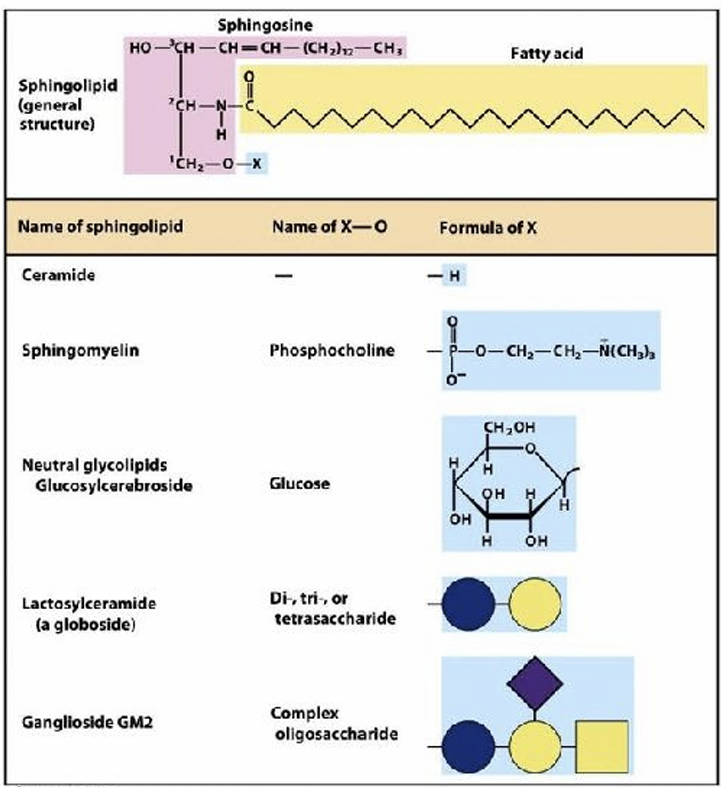
\includegraphics[width=0.5\linewidth]{sphingolipids_overview.png}
    \caption{sphingolipid structural overview}
    \label{fig:enter-label}
\end{figure}
sphingolipids all contain \textbf{cermide backbone} and a variable head group. An example of such head group is phosphocholine which produces\textbf{ sphingomyelin, the most abundant sphingolipid in mammals}. Ceramide can be \textbf{glycosilated to produce various glycosphingolipids}

\subsubsection{ceramide sythesis}
\begin{figure}[H]
    \centering
    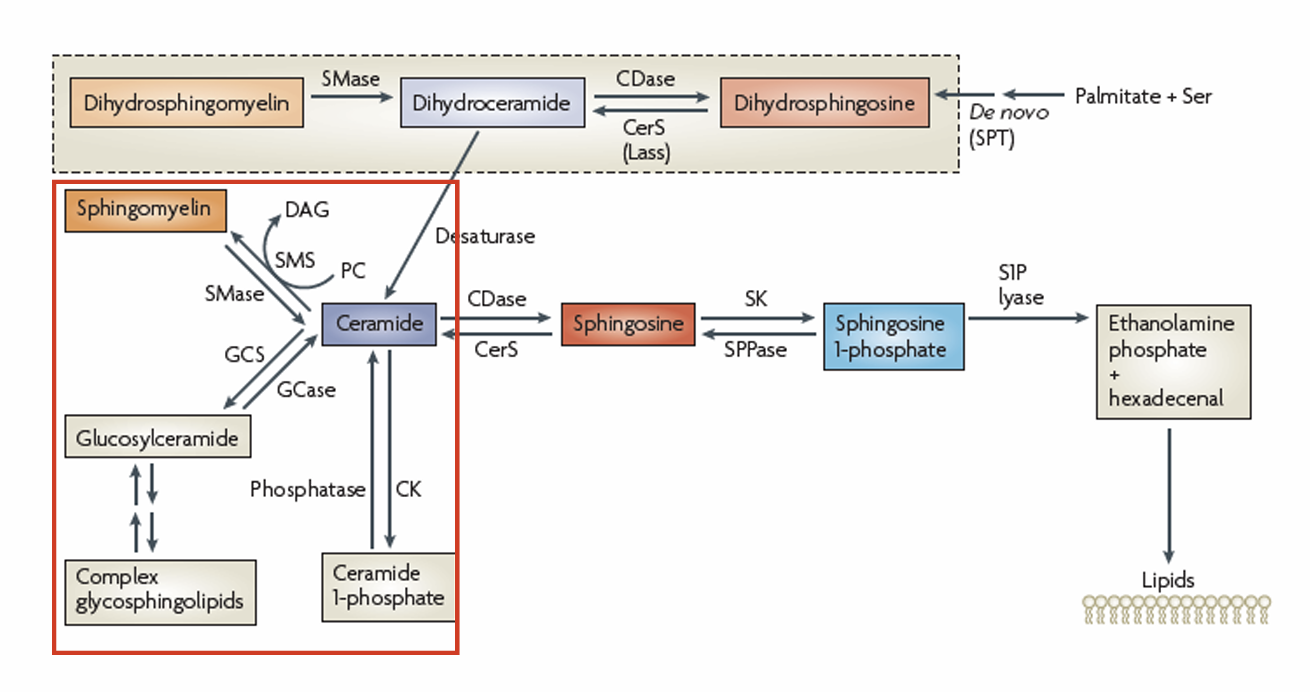
\includegraphics[width=0.7\linewidth]{overviewSphingolipidsSythesis.png}
    \caption{overview of de novo(grey box) and salvage pathway(red box)}
    \label{fig:enter-label}
\end{figure}
Ceramide being the precursor of many sphingolipids can be created in two ways, the \textbf{salvage pathway} and the \textbf{de novo pathway}.

\paragraph{de novo pathway}
\subparagraph{step1 - condensation}
\begin{figure}[h]
    \centering
    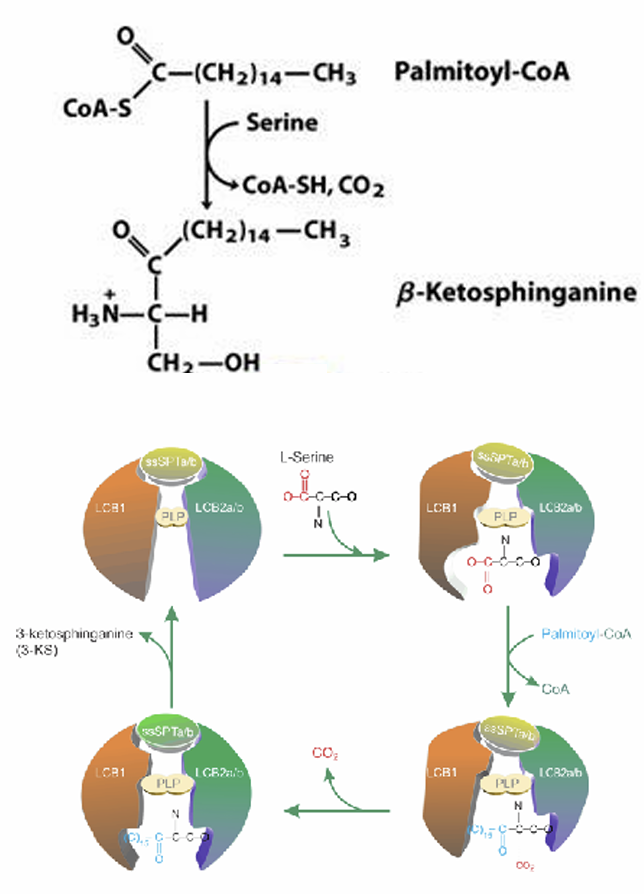
\includegraphics[width=0.5\linewidth]{step1S.png}
    \caption{step 1 - condensation}
    \label{fig:enter-label}
\end{figure}
serine and a palmitoyl-CoA 
molecule are condensed by \textbf{\gls{spt}} to form 
\textbf{$\beta$-ketosphinganine} with the \textbf{release of a CO2 molecule. }
\begin{enumerate}
    \item SPT uses pyridoxal 5'-phosphate (PLP) as a cofactor.
    \item PLP initially binds to an active-site lysine residue.
    \item L-serine displaces the lysine, forming a serine-PLP intermediate.
    \item The serine-PLP intermediate attacks palmitoyl-CoA.
    \item Following decarboxylation, $\beta$-ketosphingosine is released.
    \item PLP is regenerated in its catalytically active form.
\end{enumerate}
In \textbf{eukaryotes, SPT is a heterodimer} \textbf{localized to the endoplasmic reticulum} with The active site faces the cytosol.
--> \textbf{this is the rate limiting step }
\begin{figure}[H]
    \centering
    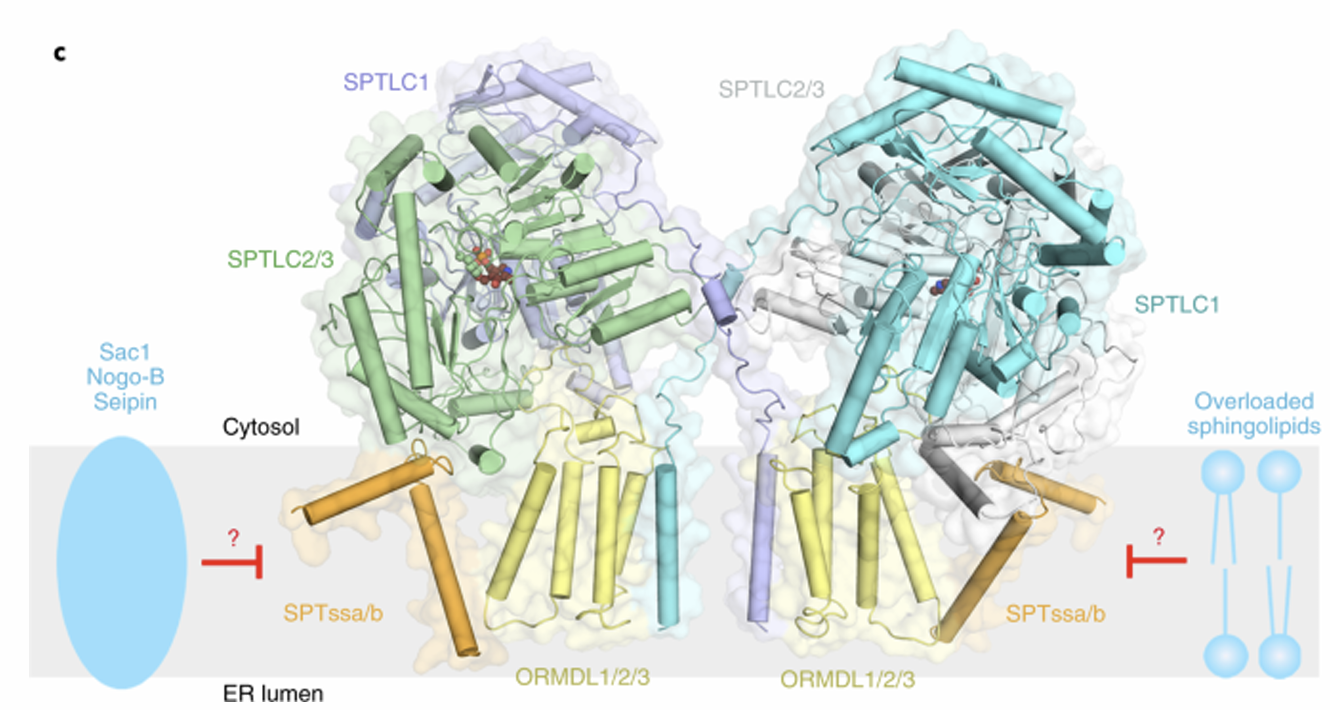
\includegraphics[width=0.5\linewidth]{structureSphingolipidSythase.png}
    \caption{serine-palmitoyltransferase (SPT)}
    \label{fig:enter-label}
\end{figure}
The \textbf{SPT enzyme is homeostatically regulated} (too high -> lower it, too low -> raise it). Among other things it pocesses an \textbf{\gls{ormdl}} domain. These are responsible for \textbf{sensing the amount of ceramide} and create a \textbf{negative feedback loop}.

\subparagraph{step2 - reduction}
\begin{figure}[H]
    \centering
    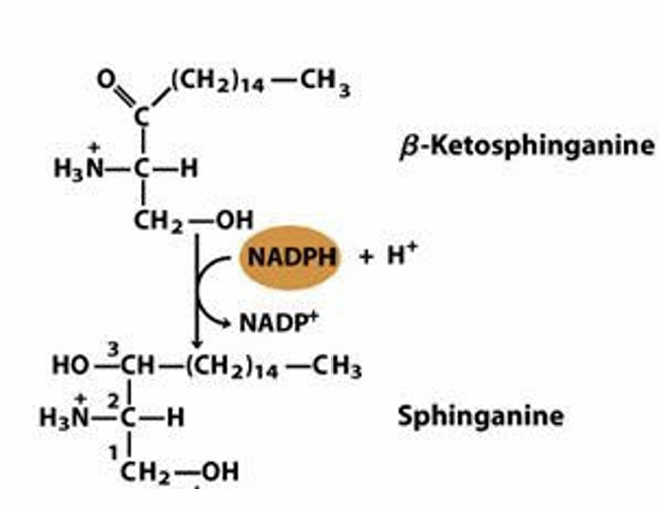
\includegraphics[width=0.5\linewidth]{step2S.png}
    \caption{step 2 - reduction}
    \label{fig:enter-label}
\end{figure}
$\beta$-ketosphingosine is reduced to 
sphinganine by \textbf{\gls{kdsr}} with 
consumption of an NADPH molecule.  
KDSR is an ER membrane protein and 
has its active site  is \textbf{oriented towards the 
cytoplasmic leaflet}.

\subparagraph{step3 - condensation}
\begin{figure}[H]
    \centering
    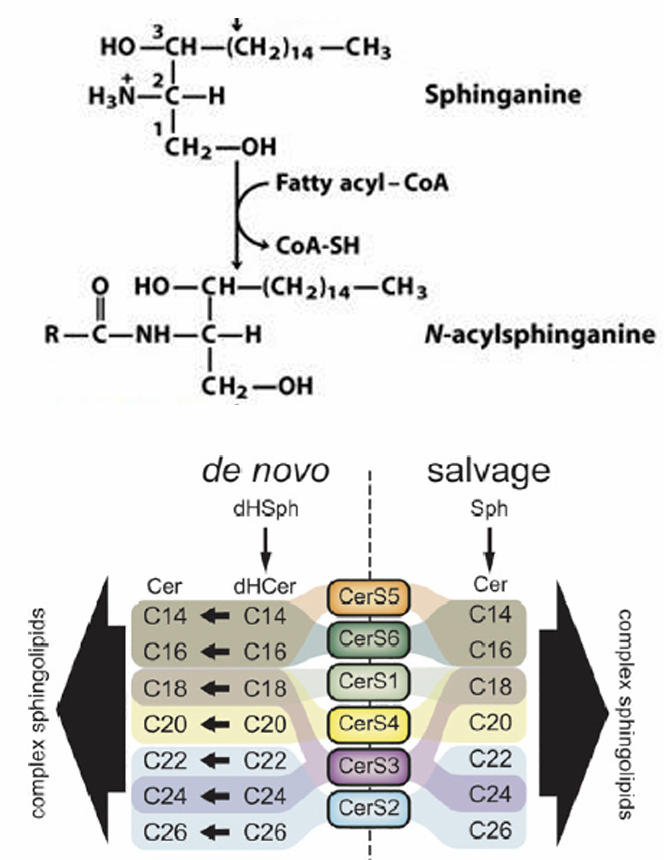
\includegraphics[width=0.5\linewidth]{step3S.png}
    \caption{step 3 - condensation}
    \label{fig:enter-label}
\end{figure}
\textbf{sphinganine} is condensed with a \textbf{fatty 
acyl-CoA} to produce \textbf{N-acylsphinganine } with \textbf{release of a free CoA}
molecule. This reaction is catalyzed by \gls{ceramidesynthase}. There are 6 ceramide sythases (CerS1-6). Each with individual substrates:
\begin{itemize}
    \item CerS2 prefers very long-chain acyl-CoAs (C22–C24–C26).
    \item CerS4 prefers C20 acyl-CoAs.
    \item CerS5 prefers shorter chains (C14–C16–C18).
\end{itemize}
\subparagraph{step4 - desaturation}

\begin{figure}[H]
    \centering
    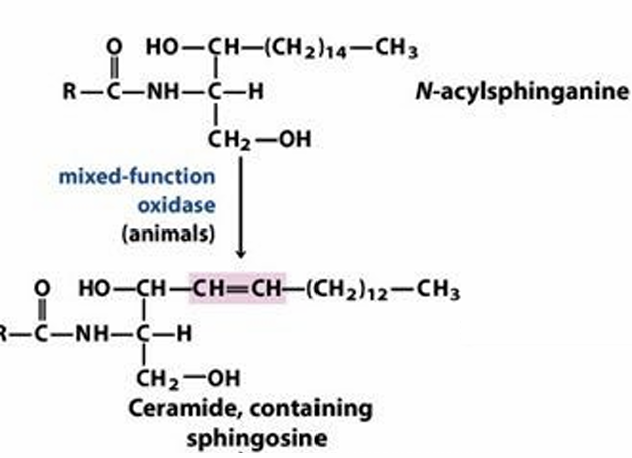
\includegraphics[width=0.5\linewidth]{step4S.png}
    \caption{step 4 - desaturation}
    \label{fig:enter-label}
\end{figure}
N-acylsphinganine (dihydroceramide) 
is desaturated to ceramide by \textbf{\gls{des}}. DES requires the \textbf{O2 and NADPH as cofactors} to add a\textbf{ 4,5-trans-double to  N-acylsphinganine.}


\paragraph{salvage pathway}
\begin{figure}[H]
    \centering
    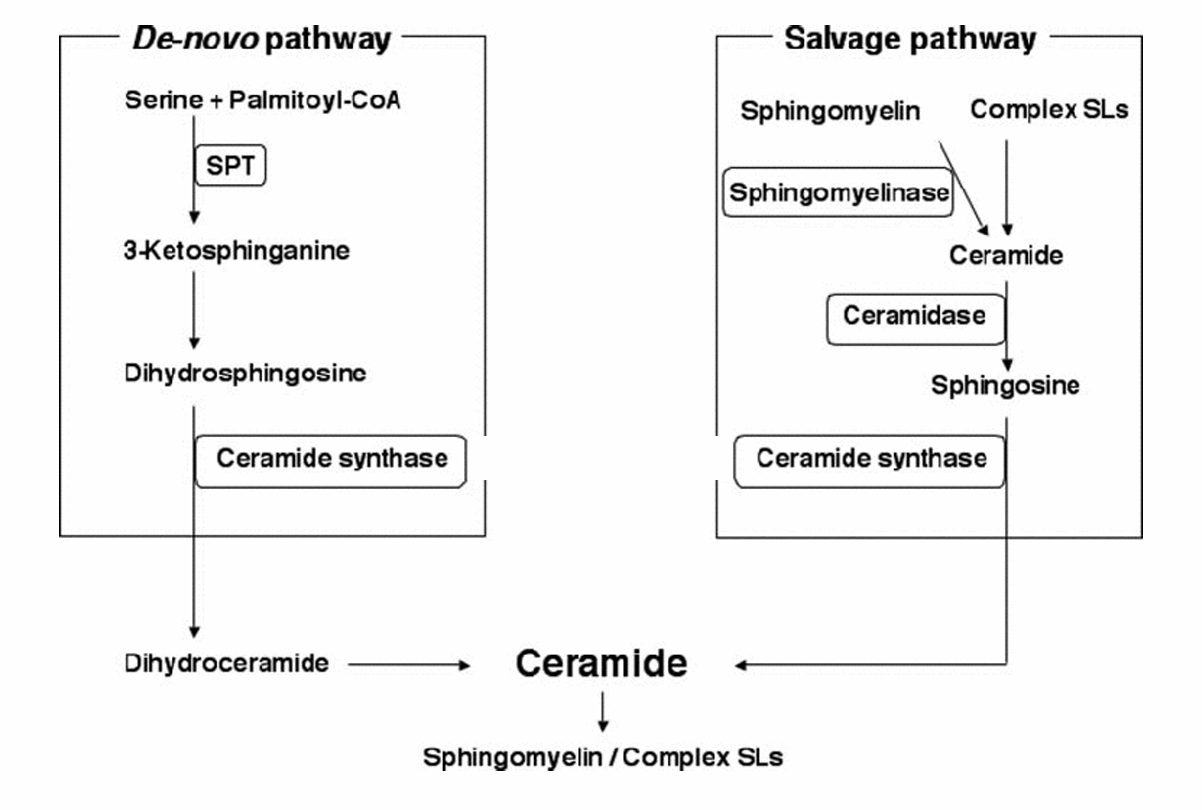
\includegraphics[width=0.7\linewidth]{2pathways.png}
    \caption{The salvage pathway (right) : Note that Ceramide is converted to Shingosine for the transport from \textbf{lisosome to the ER}}
    \label{fig:enter-label}
\end{figure}
The salvage pathway involves the production of ceramide throught the cleavage of the head group from other sphingolipids.

\subsubsection{sphingomyelin sythesis}
\begin{figure}[H]
    \centering
    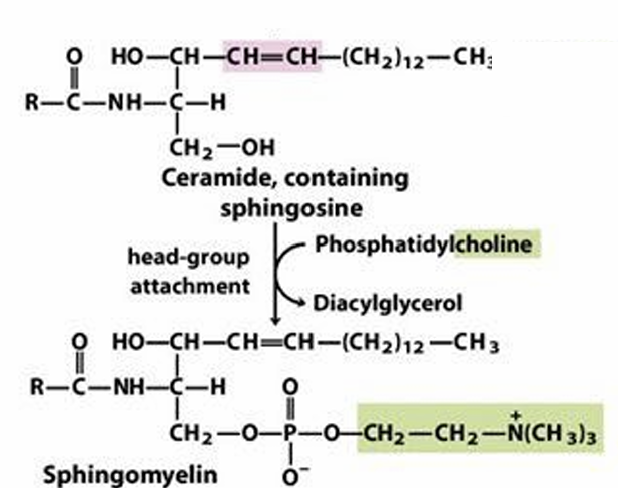
\includegraphics[width=0.5\linewidth]{sphingomyelinSythesis.png}
    \caption{sphingomyelin sythesis}
    \label{fig:enter-label}
\end{figure}
ceramide can be converted into sphingomyelin by the \textbf{\gls{sms}}. This is a\textbf{ multispan membrane protein located in the trans golgi lumen} that transfers \textbf{phosphocholine onto ceramide}. This has \textbf{diacylglycerol as a byproduct}


\paragraph{ceramide transport to golgi via cert1}
\begin{figure}[H]
    \centering
    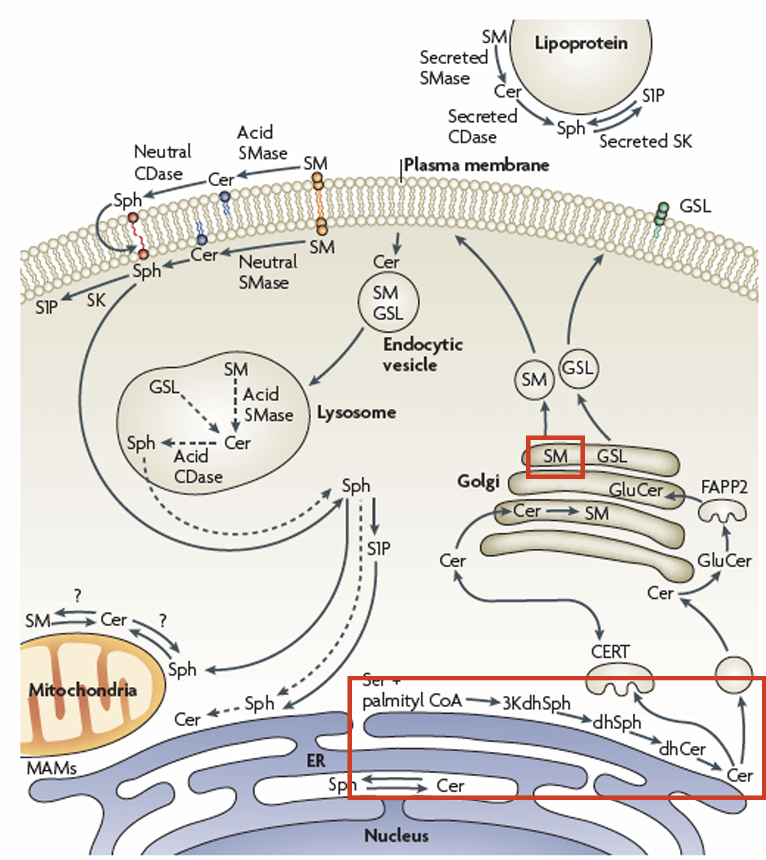
\includegraphics[width=0.5\linewidth]{topologyProblem.png}
    \caption{transporting ceramide to trans golgi lumen}
    \label{fig:trasport}
\end{figure}
\textbf{Ceramide is sythesized in the ER.} However the \textbf{active site of SMS is located in the Lumen of the trans golgi} compartment. This means that cermaide needs to be transported to the SMS active site. Since it can't diffuse through the cytoslic enviroment as this is highly unfavorable it needs to be activly transported \textbf{from ER to the lumen trans golg}i compartment by \textbf{\gls{cert1}}
\begin{figure}[H]
    \centering
    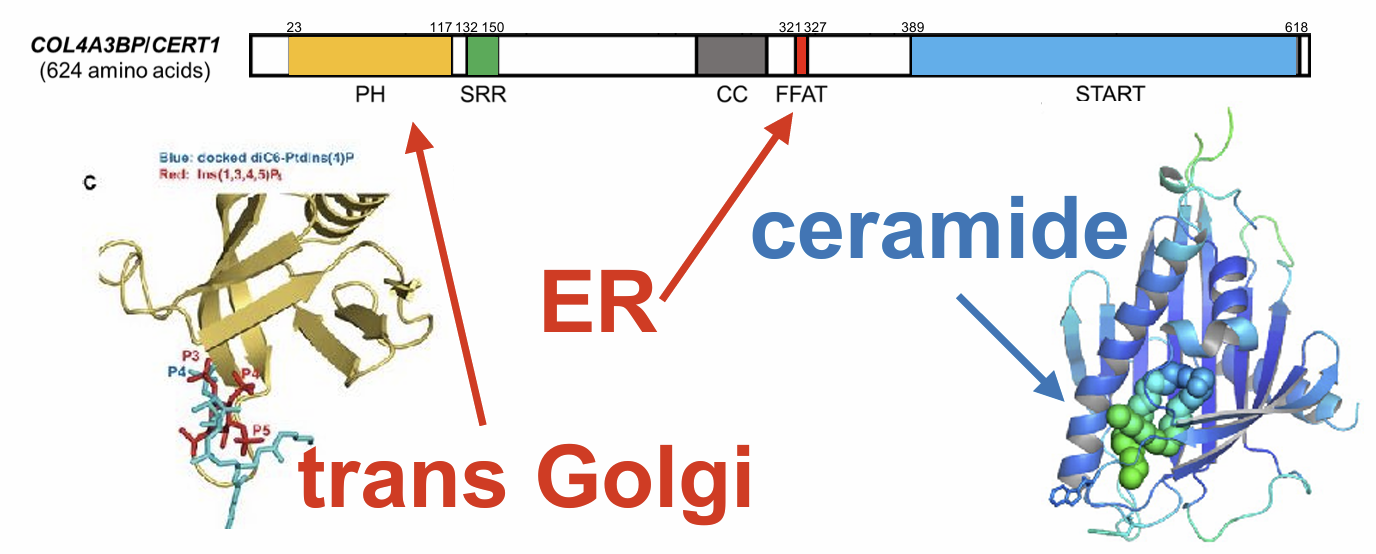
\includegraphics[width=0.5\linewidth]{cert1.png}
    \caption{cert1 structure and domains}
    \label{fig:enter-label}
\end{figure}
cert1 is a cytosolic protein that has an N-terminal \textbf{\gls{phdomain}} that will bind to \textbf{PtdIns(4)P on golgi membrane}. It also has a \textbf{\gls{ffat}} that will bind to ER membrane protein \textbf{\gls{vap}.} A \textbf{\gls{startdomain}} allows cert to bind to cermide so it can be transported to Golgi lumen. CERT1 operates ceramide transfer at 
ER-trans Golgi-\textbf{\gls{mcs}}
\begin{figure}[H]
    \centering
    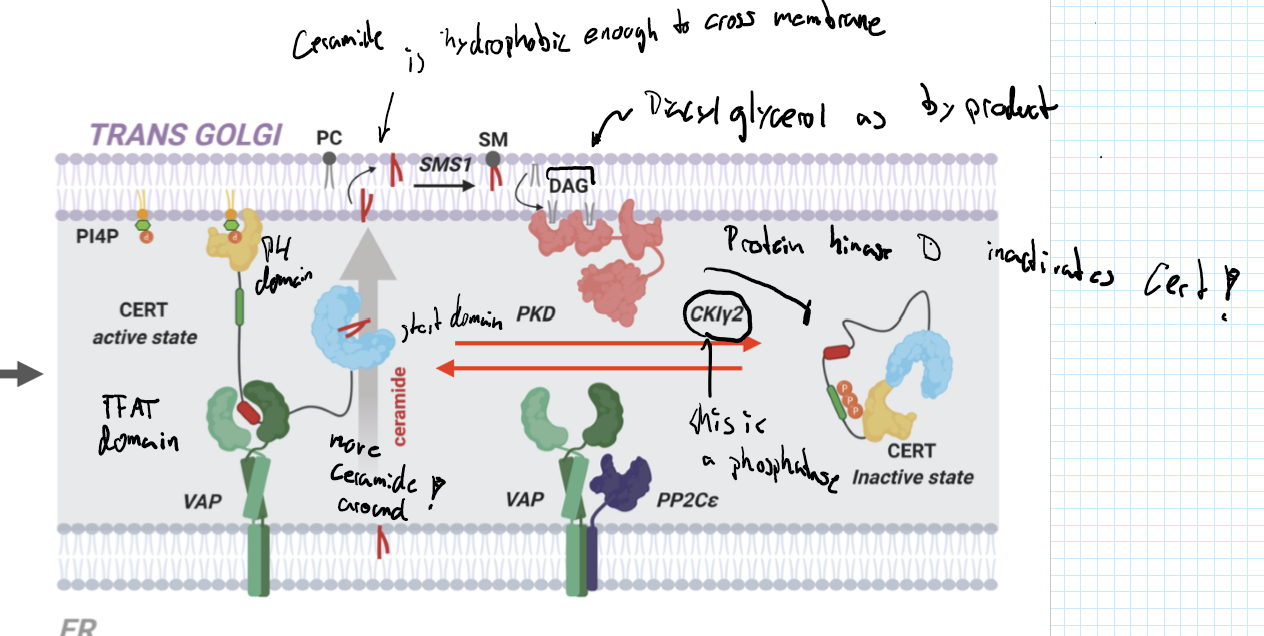
\includegraphics[width=\linewidth]{cert1_2_annotated.png}
    \caption{cert1 and it's negative feedback loop}
    \label{fig:enter-label}
\end{figure}
(there is a normal image to this aswell but in the lecture he spoke a lot about it and I feel like the anoted version might help. LMK :) )
Cert is tighly regulated and has a negative feedback loop, where if there is too much ceramide it will be phosphorylated by \textbf{PKD} which will inactivate it (homeostatic mechanism). \textbf{CKly2} will dephosphorylate it and inativate it once again if there is too little ceramide in the golgi. Sicne cert is involved in regulating sphingomyelin sythesis if mutated this will cause many \textbf{intellectual disabilities} (more than those caused by writing this shit at 2AM in a room that smells like a years supply of weed) as \textbf{sphingomyelin is a keep component of the myelinsheaths}

\subsubsection{glucosylceramide (cerebroside) sythesis}

Cermide can also be converted into \textbf{glucosylceramide (GlcCer)} also known as \textbf{\gls{cerebroside}} by \textbf{\gls{gcsc}}. Cerebroside sythesis happens on the\textbf{ cytosolic leaflet of the cis-golgi compartment} This is a key difference to that of sphingomyelin. There is \textbf{no need for speciallized transporter like Cert1} in the case of sphingomyelin production. Here simple vesicles will do the trick! (see fig. \ref{fig:trasport}). \textit{Cert1 will actually force the production of sphingomyelin by delivering directly to the trans golgi compartment}. After GlcCer has been produced it will be \textbf{translocated to the trans-golgi compartment by \gls{fapp2}.}
\paragraph{transporting from cis to trans golgi via FaPP2}
\begin{figure}[H]
    \centering
    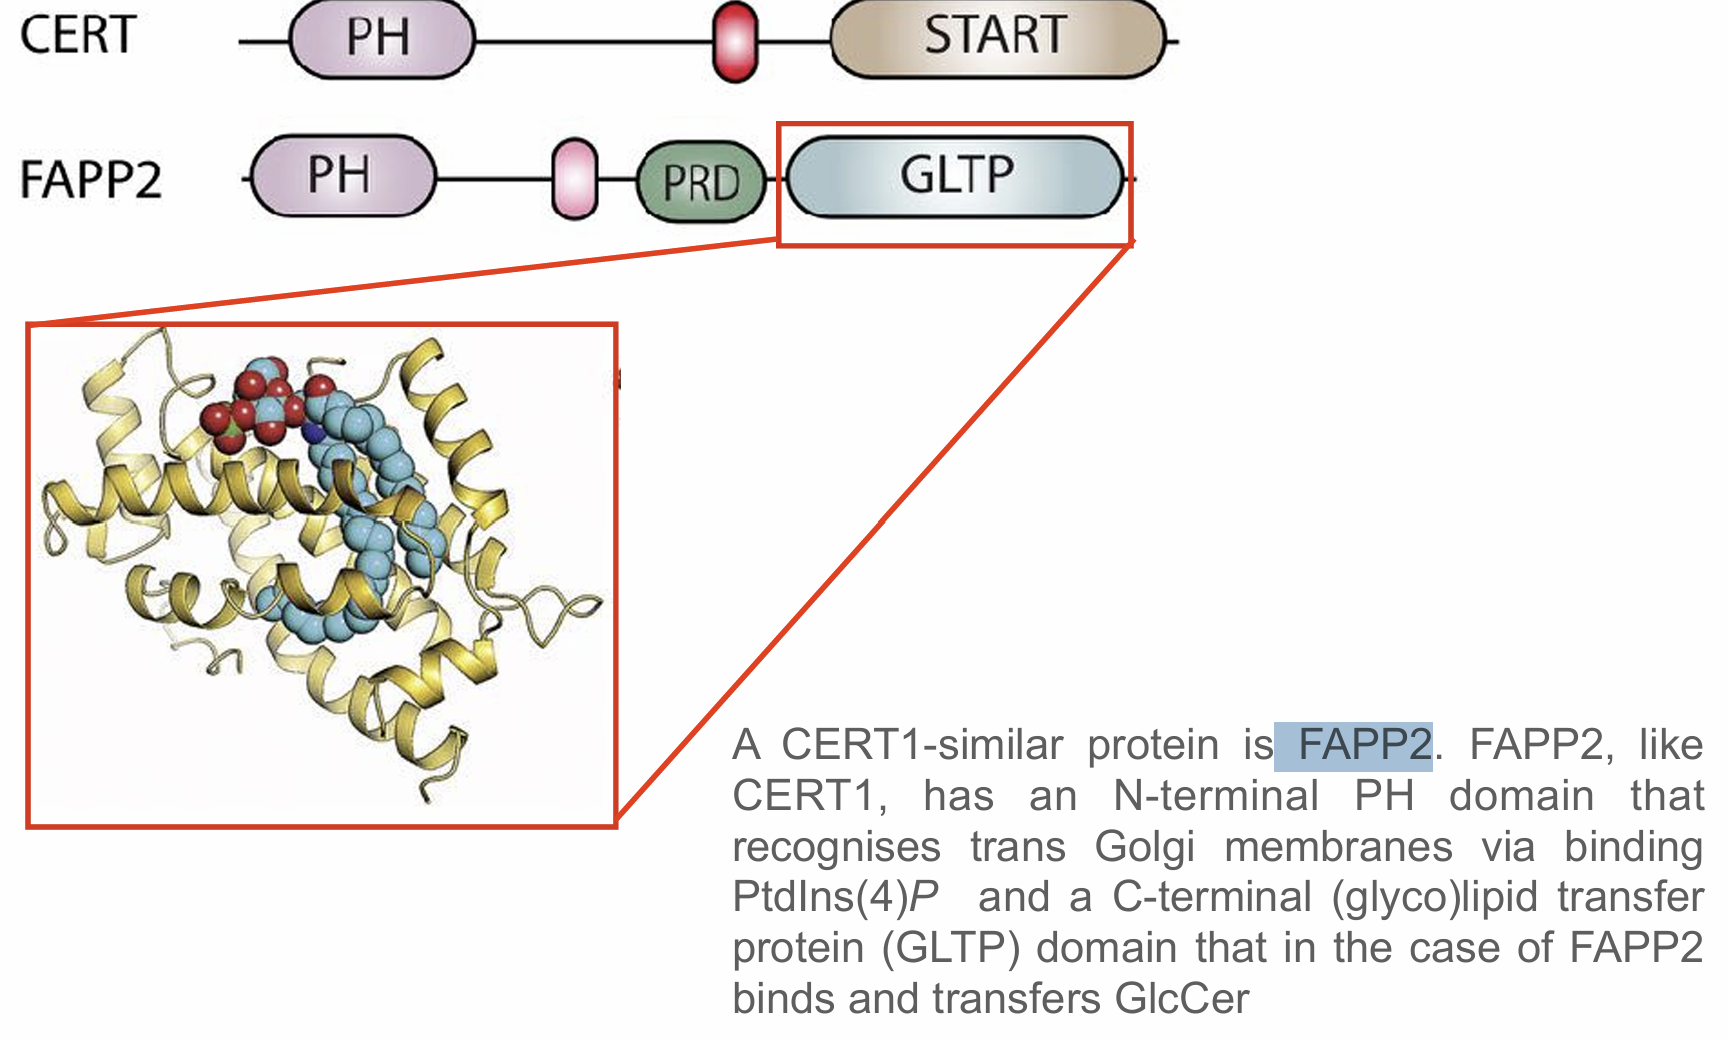
\includegraphics[width=0.5\linewidth]{FAPP2.png}
    \caption{FAPP2 domains}
    \label{fig:enter-label}
\end{figure}
this transporter also has a \gls{phdomain} to recognize the golgi via \textbf{PtdIns(4)P } binding which is located in the golgi membrane on the cytosolic leaflet side. It has a \gls{gltp} which analogously to the START domain of Cert1 will be used to bind cerebroside (GLcCer). \textbf{FAPP2 translocation to trans golgi compatment will actually seal the fate of the sphingolipid and what it can be turned into}: 
\begin{itemize}
    \item FAPP2 --> will be processed to \textbf{Globo series glycoshingolipids}
    \item if it gets to trans golgi on its own --> \textbf{Ganglio series glycosphingolipids} production
\end{itemize}
\begin{figure}[H]
    \centering
    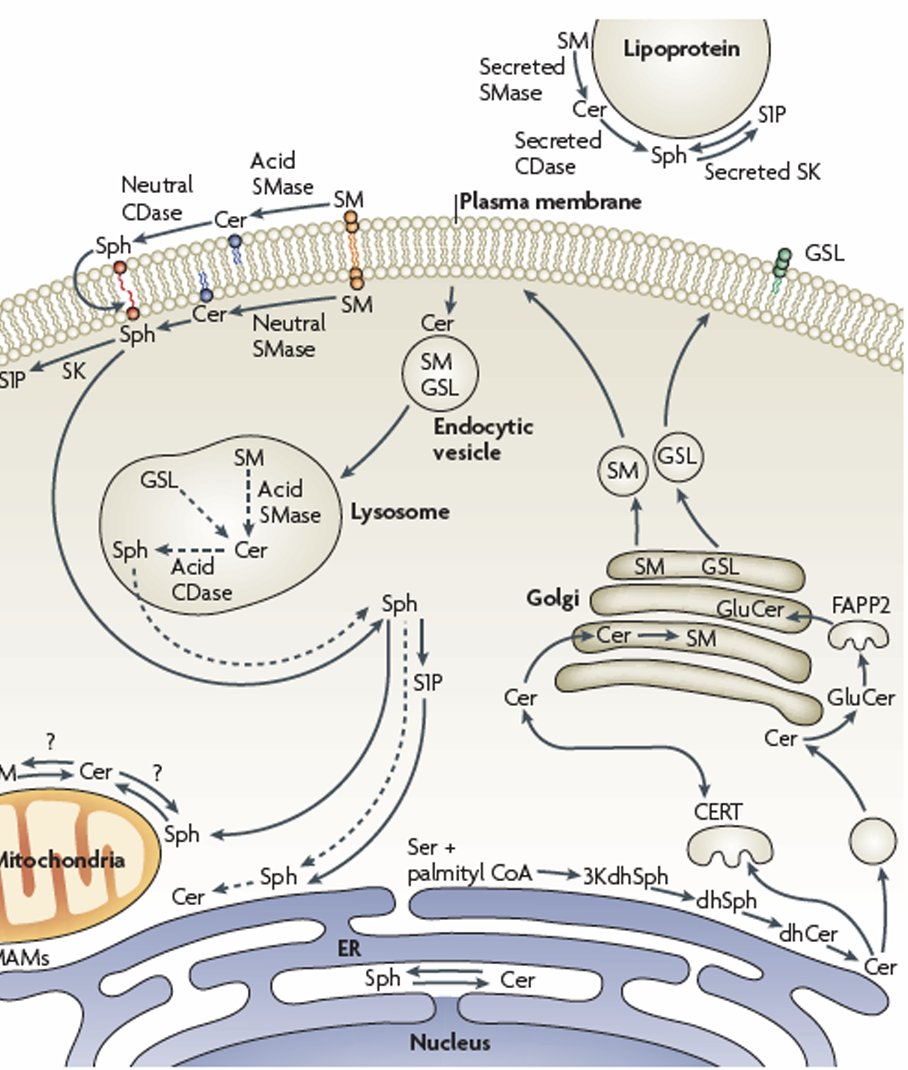
\includegraphics[width=0.4\linewidth]{transport.png}
    \caption{overview of transport pathways}
    \label{fig:enter-label}
\end{figure}

\section{Phosphoinositides}
\begin{figure}[H]
    \centering
    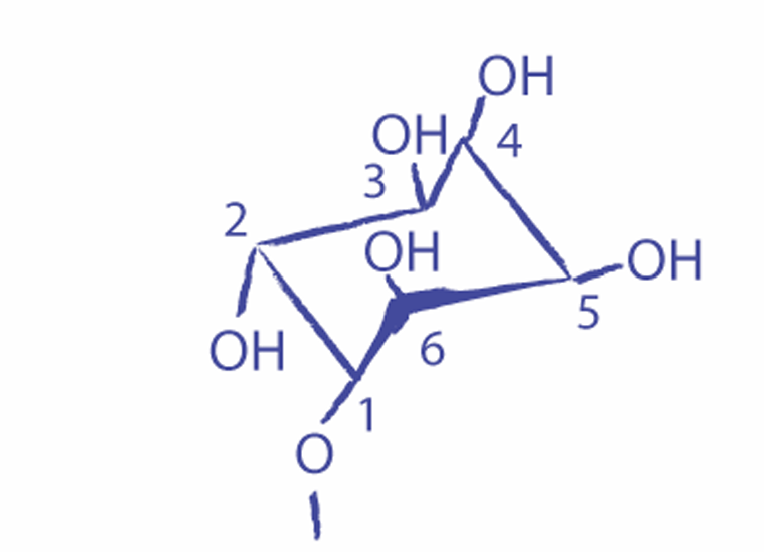
\includegraphics[width=0.3\linewidth]{inositol.png}
    \caption{inositol}
    \label{fig:enter-label}
\end{figure}
These are derived via phosphorylation of phosphatiydl inositol (ptdIn) that are produced via \textbf{\gls{phosphatidylinositol_synthase}} (see section on glycerphospholipid sythesis)

\begin{figure}[H]
    \centering
    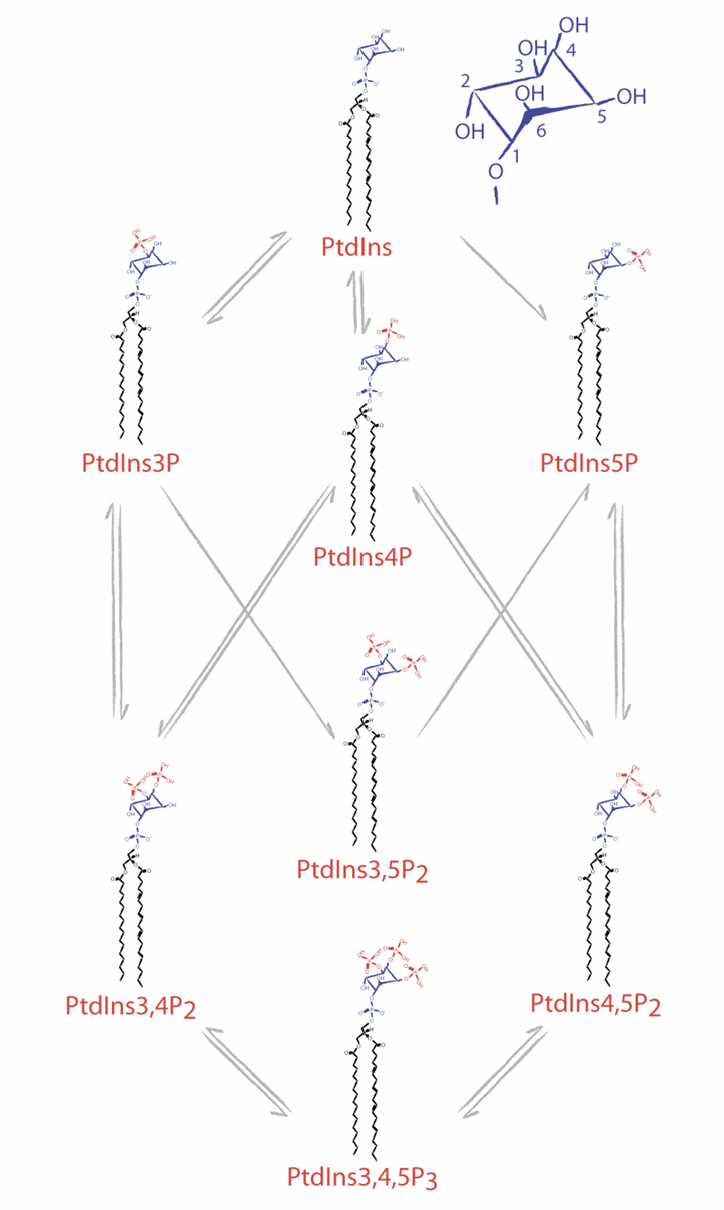
\includegraphics[width=0.3\linewidth]{PI_combinations.png}
    \caption{the 7 phosphoinositides (PI)}
    \label{fig:enter-label}
\end{figure}

\textbf{phosphorylation occurs at three, four and five hydroxyl} However, \textbf{the two and 
six hydroxyl groups are typically not 
phosphorylated} due to steric hindrance. There are about\textbf{ 50 
phosphoinositide kinases (PIKs and 
phosphatases} that are present in 
practically all cell compartments.   

\subsection{ phosphatidylinositol transfer proteins (PITPs)}
\gls{pitp} play a crucial role in transporting Phosphatydilinositols through the cytosol. These transporters can actually \textbf{trasport monomers of PtdIns or PtdCho 
between membrane compartments.} This distribution means that ptdIn is on the \textbf{cytoslic leaflet of various organelles}

\subsection{regionalisation}
\begin{figure}[H]
    \centering
    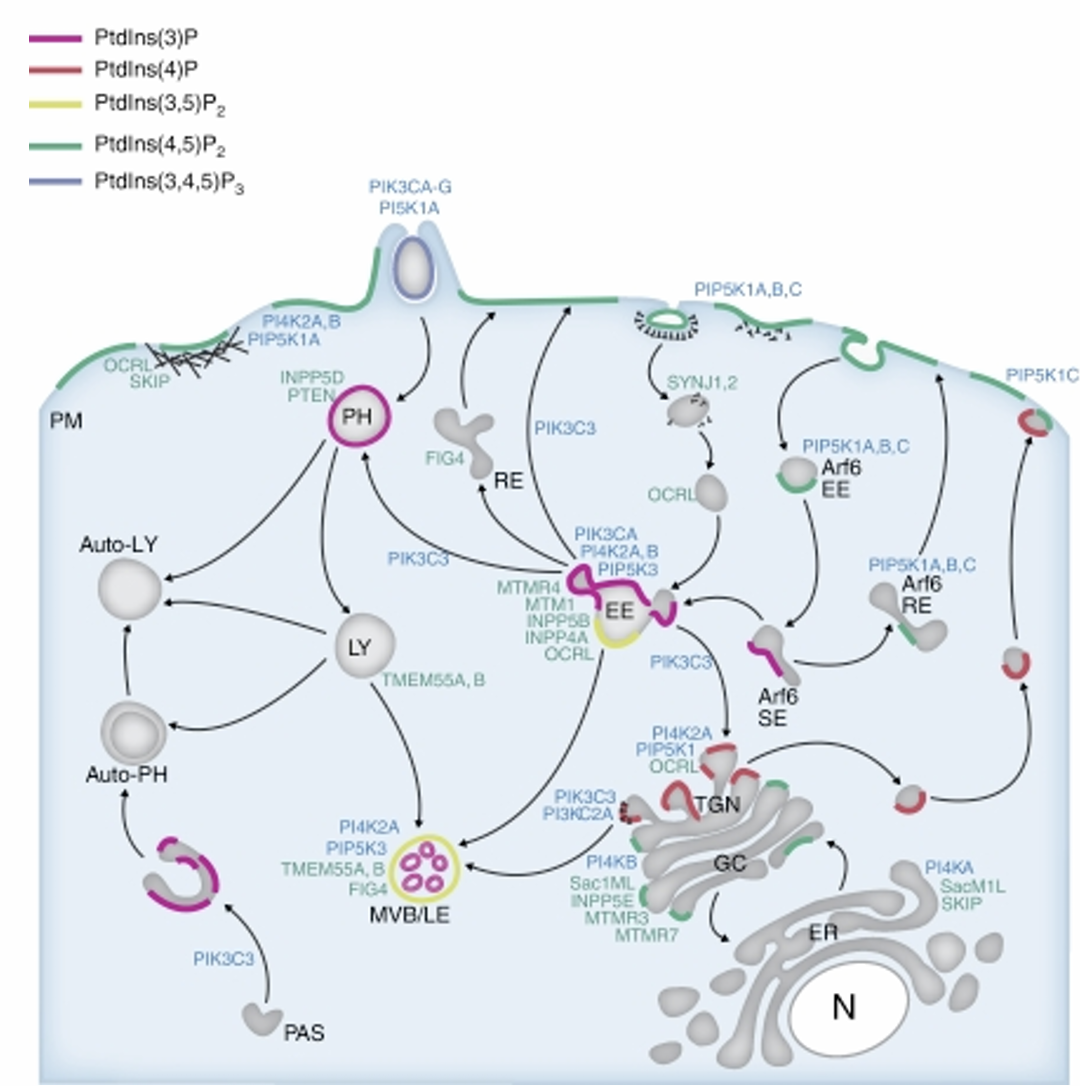
\includegraphics[width=1\linewidth]{regionalization.png}
    \caption{different phosphorylations in different compartments}
    \label{fig:enter-label}
\end{figure}
PtdIns are not distributed evenly, infact it is quite the opposite where different phosphoinositides are located in different cellular compartments. This is due to the fact that there are different PI-kinases in the different cellular compartments.  \textbf{The dynamic interplay 
between PtdIns transport and 
processing leads to lipid 
compartmentalisation.}

\subsection{recognizing membrane compartments}
Various domains recognize phosphoinositides, infact they are \textbf{ specific to the phsophorylation status of PI!.} These domains include \gls{phdomain}, \gls{FYVEdomain}, \gls{gelsolinhomologydomain}, \gls{SH2domain}, \gls{PTBdomain}. Here is an overview of a few more domains:
\begin{figure}[H]
    \centering
    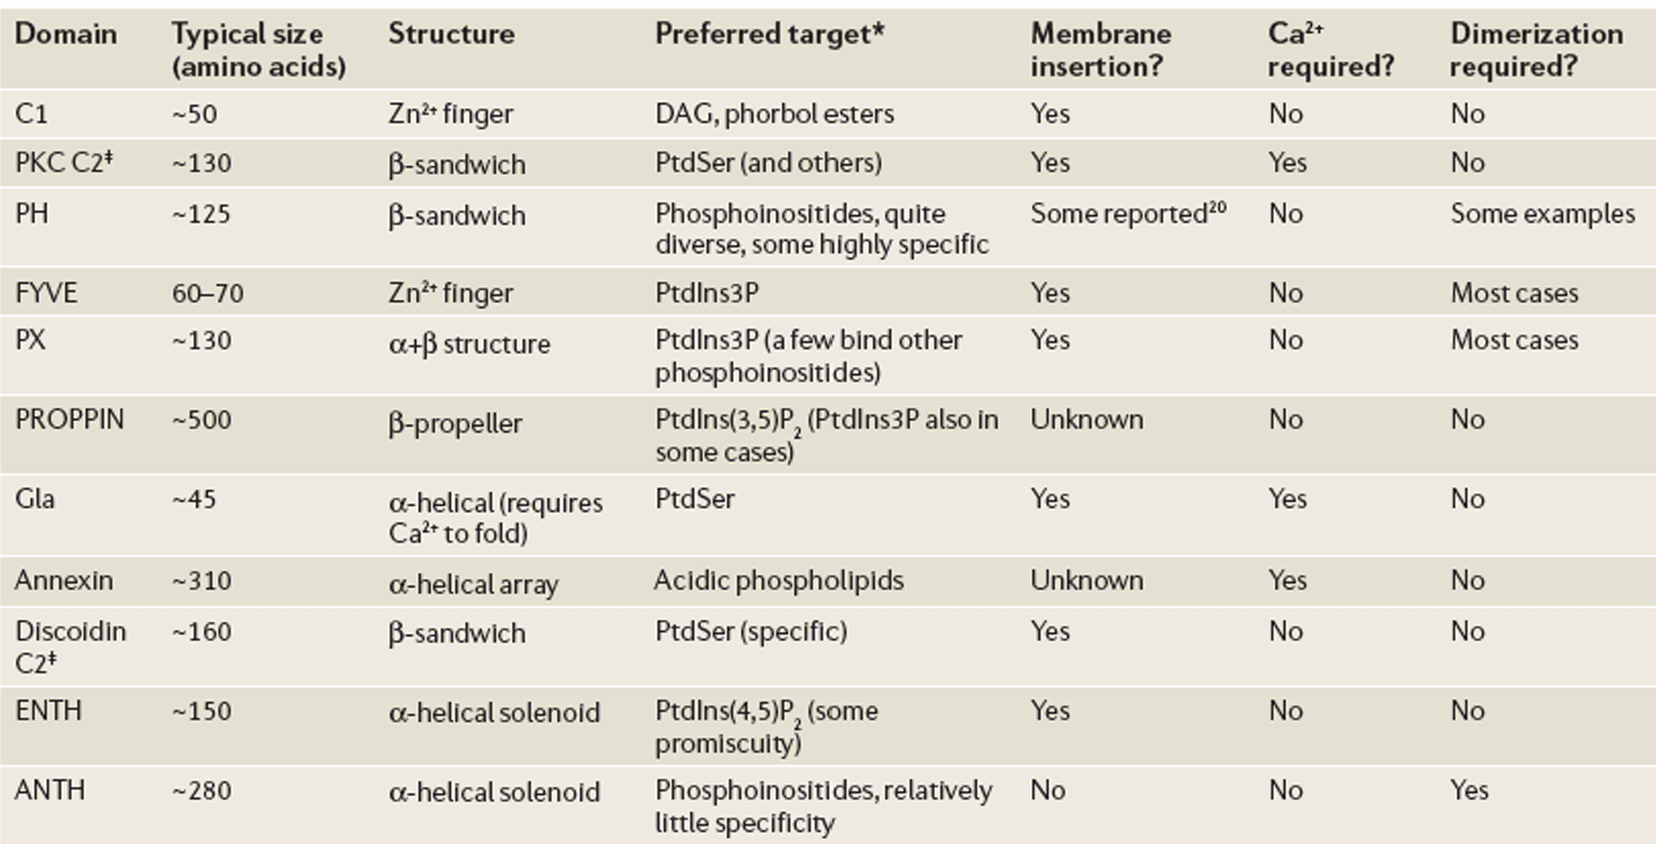
\includegraphics[width=\linewidth]{domainOverview.png}
    \caption{table of domains that recognize PIs}
    \label{fig:enter-label}
\end{figure}

typically these domains have low affinites for their binding partner. This means that they will stumble along the cytosol probing the various membrane compartments and becoming enriched in the areas where there are more of it's substrate. On top of this there is avidity \textit{(like affinity but for multible bonds at the same time)} effect, where many of these domains recognize other things as well and migh just by chance find Phosphoinositides. This is called \textbf{coincident detection}. PIs are therfore crucial for localisation of various proteins to the different organelles. \textbf{They encode the organelle's identity}

\subsubsection{PtdIns(4)P example of lipid transport coordinator}
PtdIns(4)P is the most \textbf{abundant of the monophosphorylated  
phosphoinositides.} It is produced by ptdIn phosphorylation by \textbf{\gls{PI4Ks}} which are active in the golgi. PtdIns(4)P are dephosphorylated by \textbf{\gls{Sac1} }which is active in the ER. 

--> \textbf{more PtdIns(4)P in trans golgi than ER}
\begin{figure}[H]
    \centering
    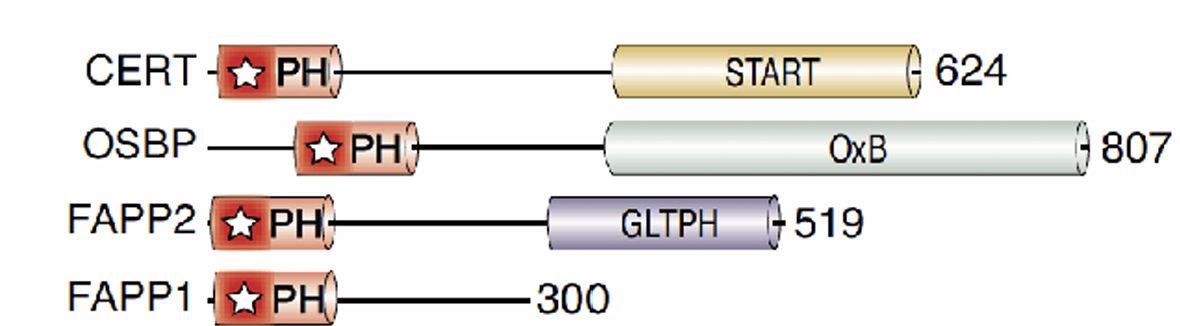
\includegraphics[width=0.5\linewidth]{moreDomainShit.png}
    \caption{domains that recognize PtdIns(4)P on trans golgi}
    \label{fig:enter-label}
\end{figure}
Various domains such as \gls{cert1}, \gls{fapp2} or \gls{OSBP} will transport ceramide to the trans golgi compartment.

-->  \textbf{PtdIns(4)P determines the lipid 
composition of the post Golgi compartments. }
\paragraph{OSBP1}
\begin{figure}[H]
    \centering
    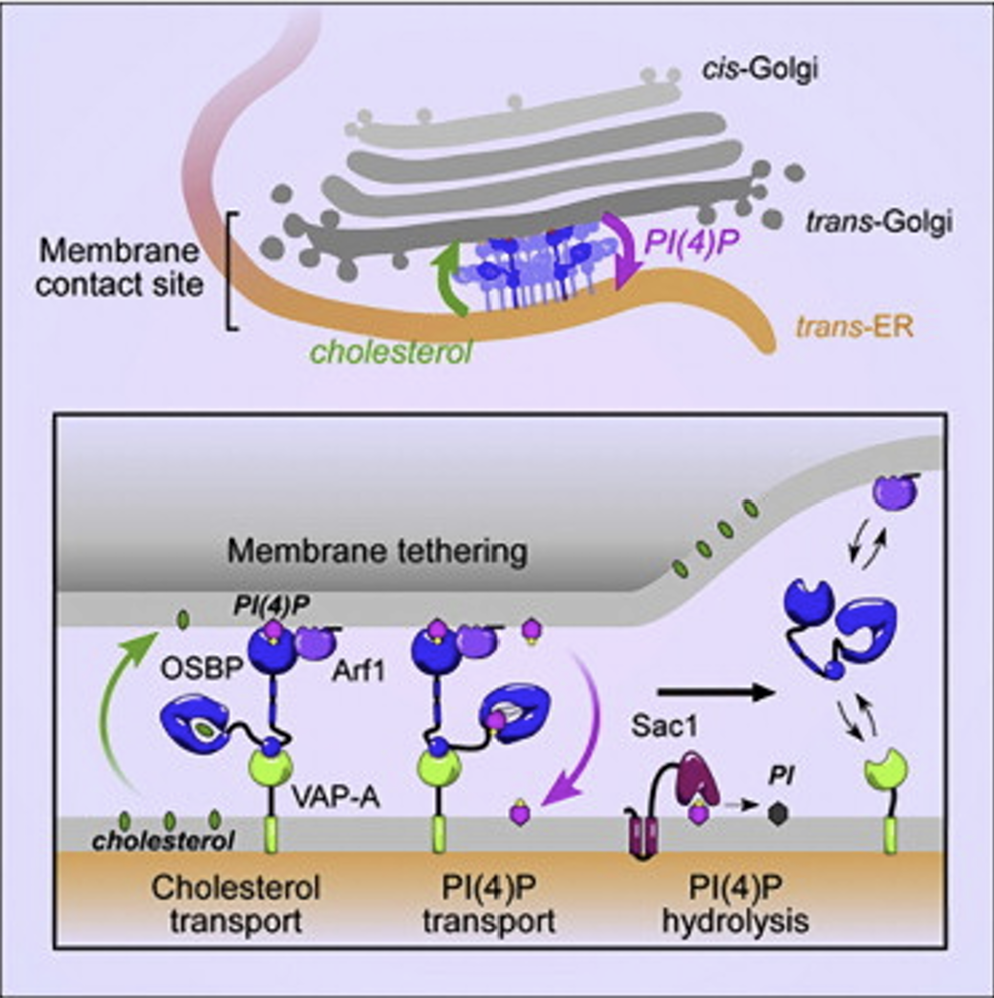
\includegraphics[width=0.5\linewidth]{OSBP1.png}
    \caption{OSBP1}
    \label{fig:enter-label}
\end{figure}
This is an interesting case for transporters as on top of transporting \textbf{cholesterol to trans golgi compartment} it wil also transport \textbf{PtdIns(4)P back to ERSac1} where it will be dephosphorylated by \textbf{\gls{Sac1}}. This is a sort of \textbf{negative feed back loop} as OSBP1  consumes its recruiting factor [i.e., PtdIns(4)P] while 
pumping cholesterol to the trans-Golgi



\subsection{PTEN and oncology relevance}
\begin{figure}[H]
    \centering
    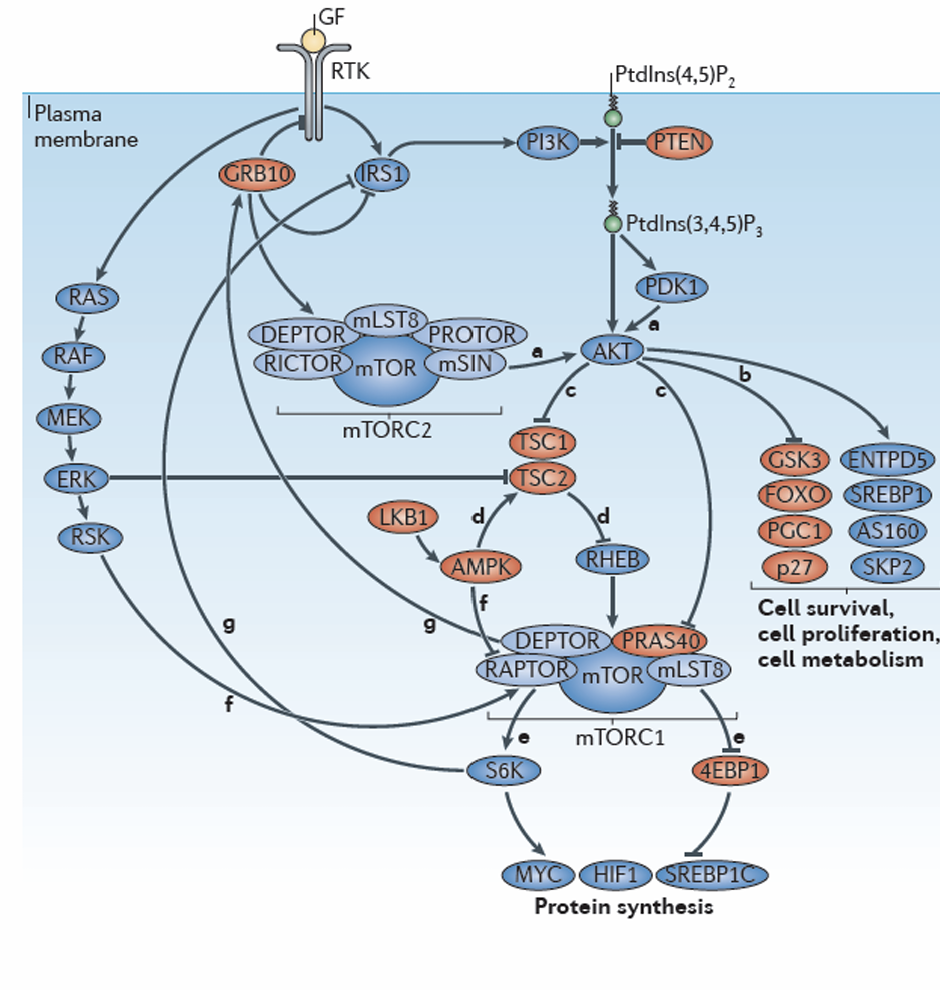
\includegraphics[width=0.5\linewidth]{PTEN.png}
    \caption{PTEN is a tumor supressor gene}
    \label{fig:enter-label}
\end{figure}
\textbf{PTEN is one of the most commonly lost tumor supressor genes.} PTEN dephosphorylates PtdIns(3,4,5)P3 to PtdIns(4,5)P2. This is the reverse of the PI3K (phosphoinositide 3-kinase) reaction, which happens in responds to a growth factor.\\
\indent It is a \textbf{phosphoinositide phosphatase}, which will reduce the effects of \textbf{PI3k}. If lost this leads to increased cell proliferation and reduced cell death.

\end{document}


